% !TEX TS–program = pdflatexmk
\documentclass[12pt,a4paper,oneside,openany]{article}
\usepackage[squaren]{SIunits}
%% LaTeX Preamble - Common packages
\usepackage[english]{babel}
\usepackage{setspace}

\usepackage{fancyhdr}
\pagestyle{fancy}
%\cfoot{\thepage{} – CONFIDENTIAL}


\usepackage[utf8]{inputenc} % Any characters can be typed directly from the keyboard, eg éçñ
\usepackage{textcomp} % provide lots of new symbols
\usepackage{graphicx}  % Add graphics capabilities
\usepackage{flafter}  % Don't place floats before their definition
%\usepackage{topcapt}   % Define \topcaption for placing captions above tables (not in gwTeX)
%\usepackage{natbib} % use author/date bibliographic citations
%\usepackage{babelbib}
\usepackage[backend=biber]{biblatex}
\addbibresource{n17-servo-design.bib}

\usepackage{caption}
\usepackage{subcaption}
\usepackage{enumitem}

\usepackage{amsmath,amssymb}  % Better maths support & more symbols
\usepackage{bm}  % Define \bm{} to use bold math fonts
\usepackage{esint}
\usepackage{algorithm}
\usepackage{mathenv}
%\usepackage[noend]{algorithmic}
\usepackage{algorithmicx}
\usepackage{algpseudocode}
\usepackage[usenames,dvipsnames]{color} 

\usepackage[pdftex,bookmarks,colorlinks,breaklinks]{hyperref}  % PDF hyperlinks, with coloured links
%\definecolor{dullmagenta}{rgb}{0.4,0,0.4}   % #660066
%\definecolor{darkblue}{rgb}{0,0,0.4}
\hypersetup{linkcolor=red,citecolor=blue,filecolor=blue,urlcolor=blue} % coloured links
%\hypersetup{linkcolor=black,citecolor=black,filecolor=black,urlcolor=black} % black links, for print output

\usepackage{memhfixc}  % remove conflict between the memoir class & hyperref
% \usepackage[activate]{pdfcprot}  % Turn on margin kerning (not in gwTeX)
%\usepackage{pdfsync}  % enable tex source and pdf output syncronicity

\usepackage{longtable}
\usepackage{booktabs}
\usepackage{listings}
\usepackage{nomencl}
\usepackage{todonotes}

\usepackage[noabbrev]{cleveref}

\usepackage{tablefootnote}
%\makesavenoteenv{tabular}

%\usepackage{pinoutikz}
%\usepackage{xparse}

\usepackage{tikz}
\usetikzlibrary{calc,arrows,through,backgrounds,fit,shapes.geometric,shapes.misc,plotmarks,positioning,trees,decorations.pathmorphing,decorations.markings,patterns}
% external lib for caching graphics
\usetikzlibrary{external}
\usepackage{circuitikz}
\usepackage{pgfplots}
\usepgfplotslibrary{external}
\tikzexternalize[prefix=tikz/]

%\usepackage{sagetex}

%\usepackage{anysize}
%\marginsize{2cm}{2cm}{2cm}{2cm}

\onehalfspacing

\makenomenclature
\def\nomlabel#1{\textbf{#1}\hfil}

%\newcommand{\Parameters}{\subsection*{Parameters}}
%\newcommand{\ReturnValue}{\subsection*{Return Value}}
%\newcommand{\Description}{\subsection*{Description}}
%\newcommand{\ClassName}[1]{{\tt #1}}
%\newcommand{\ReturnType}[1]{{\tt (#1)}}
%\newcommand{\Function}[1]{{\tt #1()}}
%\newcommand{\Self}{{\tt self}}

\DeclareMathOperator{\ud}{d}
\DeclareMathOperator{\udt}{\frac{d}{dt}}
%\DeclareMathOperator{\udtt}{\frac{\ud^2}{\ud t^2}}
\DeclareMathOperator{\rank}{rank}
\DeclareMathOperator{\fclamp}{clamp}
\DeclareMathOperator{\fsign}{sign}
%\newcommand{\ud}{\ensuremath{\binop{\mathrm{d}}}}
\newcommand{\vx}{\ensuremath{\mathbf{x}}}
\newcommand{\vy}{\ensuremath{\mathbf{y}}}
\newcommand{\vz}{\ensuremath{\mathbf{z}}}
\newcommand{\vu}{\ensuremath{\mathbf{u}}}
\newcommand{\vv}{\ensuremath{\mathbf{v}}}
\newcommand{\vw}{\ensuremath{\mathbf{w}}}
\newcommand{\va}{\ensuremath{\mathbf{a}}}
\newcommand{\vf}{\ensuremath{\mathbf{f}}}
\newcommand{\vt}{\ensuremath{\mathbf{t}}}
\newcommand{\vk}{\ensuremath{\mathbf{k}}}
\newcommand{\mM}{\ensuremath{\mathbf{M}}}
\newcommand{\mW}{\ensuremath{\mathbf{W}}}
\newcommand{\mJ}{\ensuremath{\mathbf{J}}}
\newcommand{\mA}{\ensuremath{\mathbf{A}}}
\newcommand{\mB}{\ensuremath{\mathbf{B}}}
\newcommand{\mH}{\ensuremath{\mathbf{H}}}
\newcommand{\vq}{\ensuremath{\mathbf{q}}}
\newcommand{\mC}{\ensuremath{\mathbf{C}}}
\newcommand{\mK}{\ensuremath{\mathbf{K}}}
\newcommand{\mP}{\ensuremath{\mathbf{P}}}
\newcommand{\mQ}{\ensuremath{\mathbf{Q}}}
\newcommand{\mR}{\ensuremath{\mathbf{R}}}
\newcommand{\mS}{\ensuremath{\mathbf{S}}}
\newcommand{\vlambda}{\ensuremath{\boldsymbol{\lambda}}}
\newcommand{\vd}{\ensuremath{\mathbf{d}}}
\newcommand{\mI}{\ensuremath{\mathbf{I}}}
\newcommand{\vc}{\ensuremath{\mathbf{c}}}
\newcommand{\vr}{\ensuremath{\mathbf{r}}}
\newcommand{\vF}{\ensuremath{\mathbf{F}}}
\newcommand{\vtau}{\ensuremath{\boldsymbol{\tau}}}
\newcommand{\valpha}{\ensuremath{\boldsymbol{\alpha}}}

\newtheorem{mydef}{Definition}


\lstset{numbers=left,basicstyle=\footnotesize\ttfamily,numberstyle=\tiny,tabsize=4,breaklines=true}
\lstset{language=[Objective]C}
\lstset{commentstyle=\color{BrickRed}\itshape,
	keywordstyle=\color{RoyalBlue}\bfseries,
	identifierstyle=\color{Blue},
	stringstyle=\color{Gray}}

\long\def\symbolfootnote[#1]#2{\begingroup%
\def\thefootnote{\fnsymbol{footnote}}\footnote[#1]{#2}\endgroup}


\begin{document}


\title{Servo Controller Design Notes}
\author{Dömötör Gulyás\\v0.1}

\maketitle

%\abstract
%
%foopsum.
%
%

\tableofcontents

%\listoffigures

%\section{Introduction}

%\begin{figure}[htbp]
%\begin{center}
%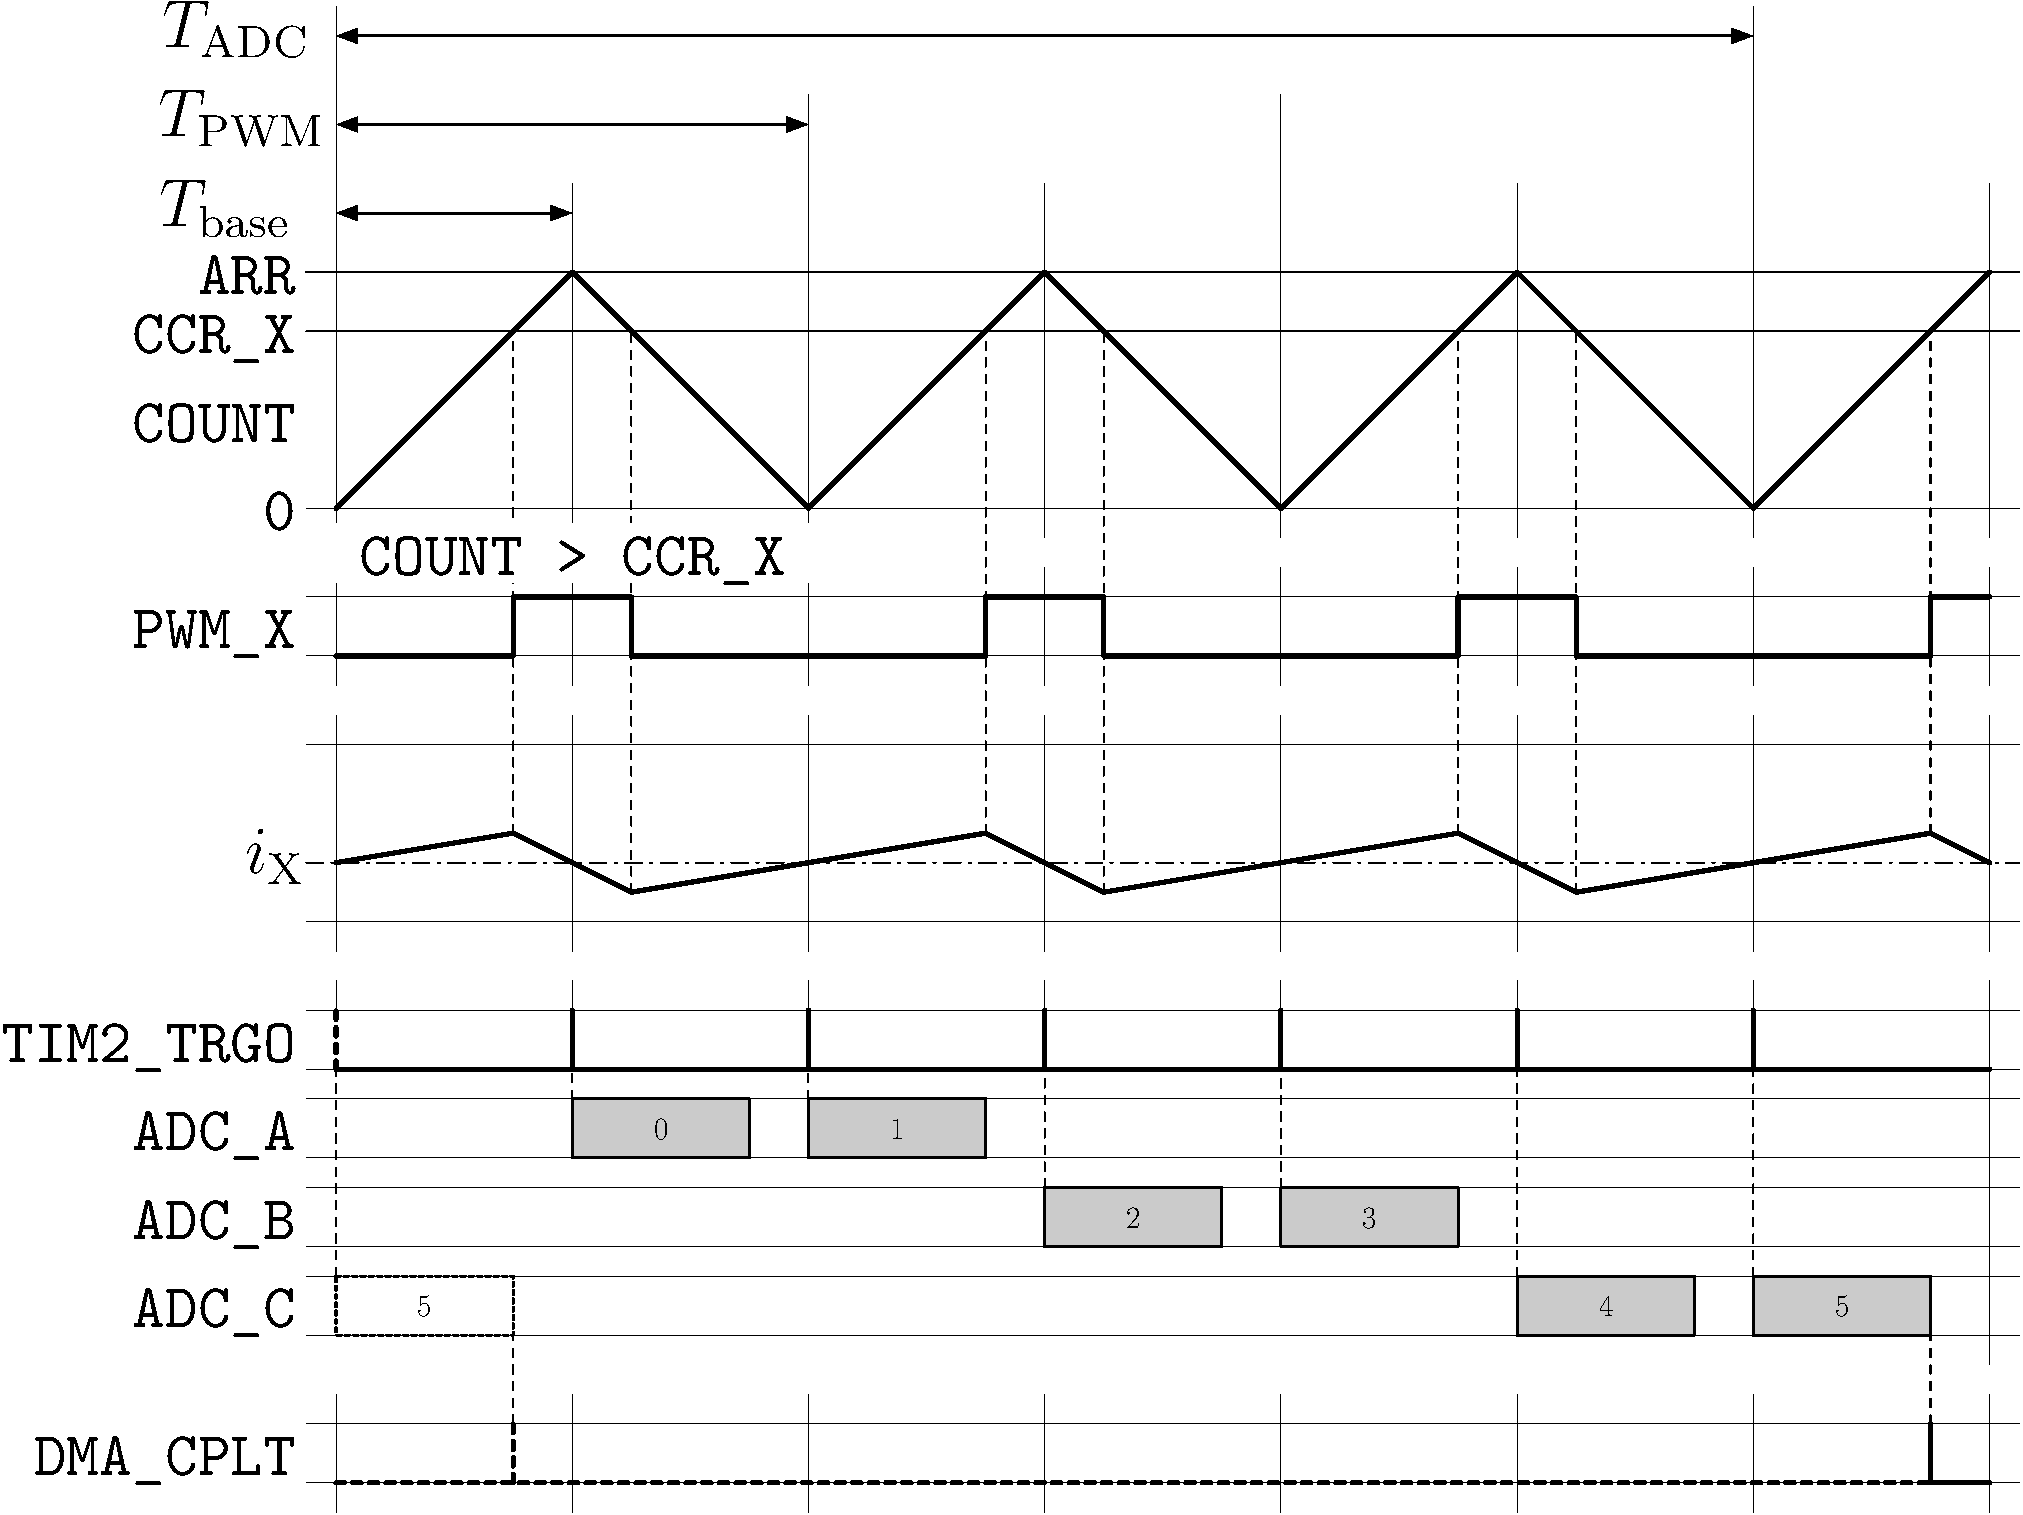
\includegraphics[scale=0.8]{n17-servo-pwm-adc.pdf}
%\caption[Fig]{foo}
%\label{fig:pwm-adc}
%\end{center}
%\end{figure}

\section{TODO}

\subsection{Flux-braking}
\href{https://en.wikipedia.org/wiki/Braking_chopper#Flux_braking}{https://en.wikipedia.org/wiki/Braking\_chopper\#Flux\_braking}


\section{Hardware}

The hardware is laid out to be as flexible as possible, driving both 3-phase BLDC and servo motors, as well as 2-phase steppers.

3 half bridges with discrete transistors allow high currents. The DRV8323 stepper driver works at up to 60V. The hardware is laid out for 12V-48V nominal voltage, but allowing 60V peak.

Using a 2-phase motor in this configuration limits the top speed due to lower effective voltage than one could get using 2 full bridges.

The main MCU is an STM32G431.

\subsection{SPI}

Unfortunately the STM32G4 SPI implementation does not allow hardware NSS signaling, as the SPI mode that needs to be used with the attached SPI devices (low clock polarity, latch on 2nd edge) is not compatible with hardware pulsing of NSS between data frames.

\subsection{MCU Peripheral Assignments}

\begin{table}[htbp]
\caption{MCU Peripheral Usage}
\begin{center}
\begin{tabular}{ll} \toprule
 Peripheral & Usage \\
\midrule \texttt{ADC1} & Auxiliary analog inputs \\
\texttt{ADC2} & Current Sensing \\
\midrule
\texttt{TIM1} & Event counter for debugging \\
\texttt{TIM2} & PWM Gate Driver (R,A,B,C) \\
\texttt{TIM3} & Encoder Input \\
\texttt{TIM4} & RGB LED PWM + SYNC\\
\texttt{TIM6} & Performance Counter / Timer \\
\texttt{TIM15} & current sense trigger offset \\
\texttt{TIM16} & SPI NSS pulse timer \\
\midrule
\texttt{I2C3} & I2C I/O \\
\texttt{USART1} & Debug I/O \\ 
\texttt{SPI2} & Gate Driver and Magnetic Encoder \\
\texttt{USB} & USB Interface \\
\bottomrule
\end{tabular}
\end{center}
\label{tab:mcu-peripherals}
\end{table}%

\begin{figure}[htbp]
\begin{center}
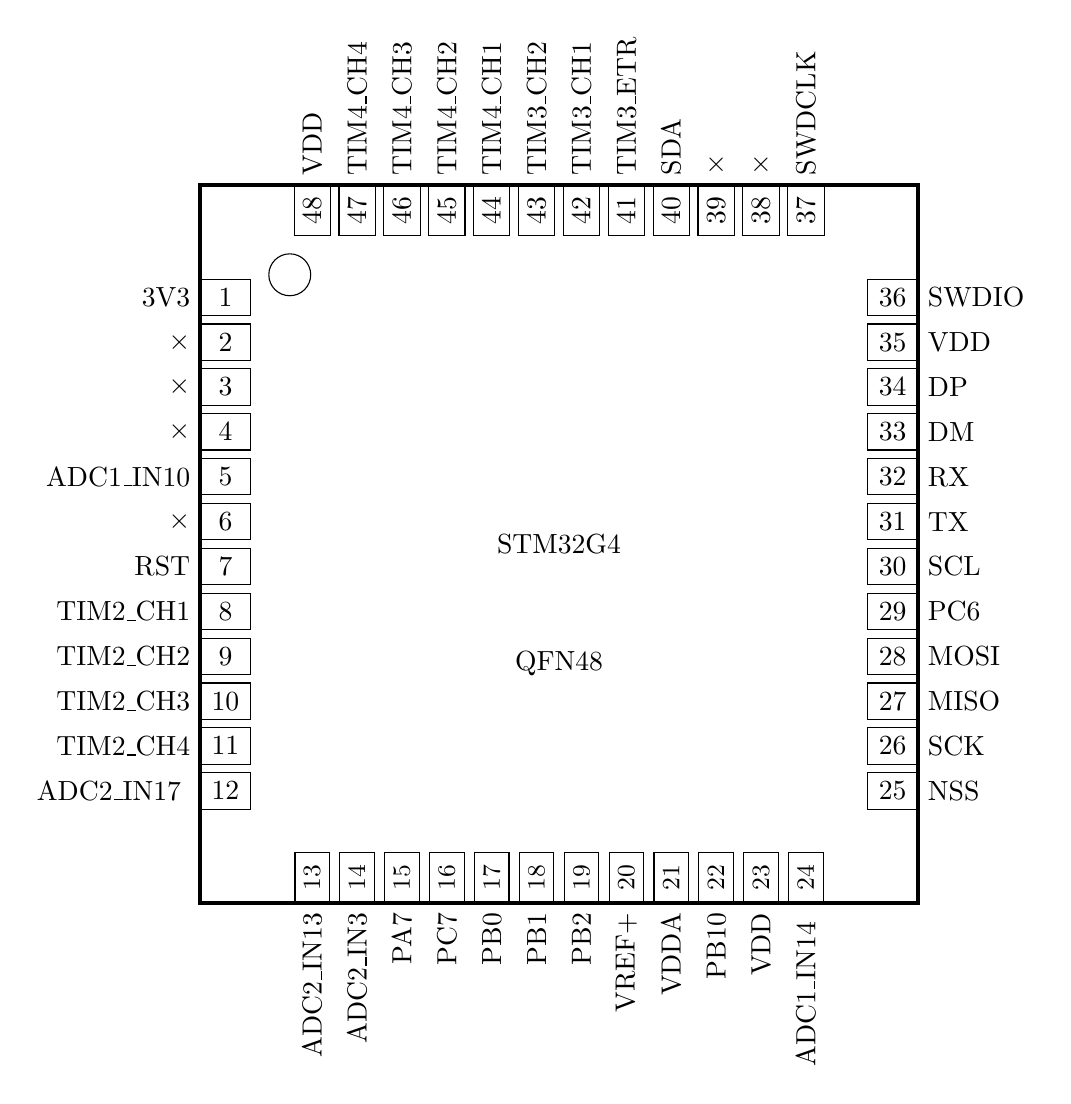
\begin{tikzpicture}[scale=0.38,
     pin/.style={draw,rectangle,minimum width=1.8em}
     ]
   % Main trick: loop over the label numbers and then adjust their position
   % in the tikzpicture using evaluate to calculate \y=y-coordinate of pin
   \foreach \i/\desc [evaluate=\i as \y using (1.5*(-\i+6.5))]
      in {1/{3V3},
          2/{$\times$},
          3/{$\times$},
          4/{$\times$},
          5/{ADC1\_IN10},
          6/{$\times$},
          7/{RST},
          8/{TIM2\_CH1},
          9/{TIM2\_CH2},
         10/{TIM2\_CH3},
         11/{TIM2\_CH4},
         12/{ADC2\_IN17} }
   {
     \draw node[pin,anchor=west] at (-12,\y){$\i$}; % pin
     \node[align=right,anchor=east] at (-12,\y){\desc}; % description
   }
   \foreach \i/\desc [evaluate=\i as \x using (1.5*((\i-12)-6.5))]
     in {13/{ADC2\_IN13},
         14/{ADC2\_IN3},
         15/{PA7},
         16/{PC7},
         17/{PB0},
         18/{PB1},
         19/{PB2},
         20/{VREF+},
         21/{VDDA},
         22/{PB10},
         23/{VDD},
         24/{ADC1\_IN14} }
   {
     \draw node[pin,anchor=west,rotate=90] at (\x,-12){\small$\i$};
     \node[align=right,anchor=east,rotate=90] at (\x,-12){\desc};
   }
   \foreach \i/\desc [evaluate=\i as \y using (1.5*((\i-24) - 6.5)]
     in {25/{NSS},
         26/{SCK},
         27/{MISO},
         28/{MOSI},
         29/{PC6},
         30/{SCL},
         31/{TX},
         32/{RX},
         33/{DM},
         34/{DP},
         35/{VDD},
         36/{SWDIO} }
   {
     \draw node[pin,anchor=east] at (12,\y){$\i$};
     \node[align=left,anchor=west] at (12,\y){\desc};
   }
   \foreach \i/\desc [evaluate=\i as \x using (1.5*(6.5-(\i-36)))]
     in {37/{SWDCLK},
         38/{$\times$},
         39/{$\times$},
         40/{SDA},
         41/{TIM3\_ETR},
         42/{TIM3\_CH1},
         43/{TIM3\_CH2},
         44/{TIM4\_CH1},
         45/{TIM4\_CH2},
         46/{TIM4\_CH3},
         47/{TIM4\_CH4},
         48/{VDD} }
   {
     \draw node[pin,anchor=east,rotate=90] at (\x,12){$\i$};
     \node[align=right,anchor=west,rotate=90] at (\x,12){\desc};
   }
%   \draw[ultra thick]
%      (0,0.8)--(0,17.2)--(0.8,18)--(17.2,18)--(18,17.2)
%             --(18,0.8)--(17.2,0)--(0.8,0)--cycle;
   \draw[ultra thick]
      (-12,-12)--(-12,12)--(12,12)
             --(12,-12)--cycle;
   \draw(-9,9)circle[radius=0.7];
   \node (mcu) at (0,0){STM32G4};
   \node[below=of mcu]{QFN48};
 \end{tikzpicture}
\caption[RL Circuit]{STM32G4 pinout diagram.}
\label{fig:stm-pinout}
\end{center}
\end{figure}


\begin{longtable}[htbp]{@{}rlll@{}}%
\caption{STM32G431 pin assignments for hardware version 0.3. \label{tab:mcu-pins}} \\
\toprule 
        Pin & GPIO         & Peripheral        & Usage \\
\midrule 
\endfirsthead
%\midrule
\multicolumn{4}{c}{\ldots table continued from previous page} \\
\midrule
         Pin & GPIO         & Peripheral        & Usage \\
\midrule
\endhead
\multicolumn{4}{c}{table continues on next page \ldots} \\
%\midrule
\endfoot
\bottomrule
\endlastfoot
          1 & \texttt{VBAT} &                   & \texttt{3V3}  \\
\midrule  5 & \texttt{PF0}  &\texttt{ADC1 IN10} & VDDP sensing \\
\midrule  7 & \texttt{PG10} &                   & reset input \\
\midrule  8 & \texttt{PA0}  &\texttt{TIM2 CH1}  & Brake Resistor PWM \\
          9 & \texttt{PA1}  &\texttt{TIM2 CH2}  & Channel A PWM \\
         10 & \texttt{PA2}  &\texttt{TIM2 CH3}  & Channel B PWM \\
         11 & \texttt{PA3}  &\texttt{TIM2 CH4}  & Channel C PWM \\
\midrule 12 & \texttt{PA4}  &\texttt{ADC2 IN17} & Current Sense Channel A \\
         13 & \texttt{PA5}  &\texttt{ADC2 IN13} & Current Sense Channel B \\
         14 & \texttt{PA6}  &\texttt{ADC2 IN3}  & Current Sense Channel C \\
\midrule 15 & \texttt{PA7}  &                   & DRV8323 Enable \\
\midrule 16 & \texttt{PC4}  &                   & DRVFAULT input \\
\midrule 17 & \texttt{PB0}  &                   & Enable Driver Channel C \\
         18 & \texttt{PB1}  &                   & Enable Driver Channel B \\
         19 & \texttt{PB2}  &                   & Enable Driver Channel A \\
\midrule 22 & \texttt{PB10} &                   & SPI Select AS5047 \\
\midrule 24 & \texttt{PB11} &\texttt{ADC1 IN14} & VBUS sensing \\
\midrule 25 & \texttt{PB12} &\texttt{SPI2 NSS}  &  \\
         26 & \texttt{PB13} &\texttt{SPI2 SCK}  &  \\
         27 & \texttt{PB14} &\texttt{SPI2 MISO} &  \\
         28 & \texttt{PB15} &\texttt{SPI2 MOSI} &  \\
\midrule 29 & \texttt{PC6}  &                   & SPI Select DRV8323 \\

\midrule 30 & \texttt{PA8}  &\texttt{I2C3 SCL}  & \\
\midrule 31 & \texttt{PA9}  &\texttt{UART1 TX}  & Debug TX \\
         32 & \texttt{PA10} &\texttt{UART1 RX}  & Debug RX \\
\midrule 33 & \texttt{PA11} &\texttt{USB DM}    & \\
         34 & \texttt{PA12} &\texttt{USB DP}    & \\
\midrule 36 & \texttt{PA13} &\texttt{SWD SWDIO} & \\
         37 & \texttt{PA14} &\texttt{SWD SWCLK} & \\
\midrule 40 & \texttt{PC11} &\texttt{I2C3 SDA}  & \\
\midrule 41 & \texttt{PB3}  &\texttt{TIM3 ETR}  & External Encoder I\\
         42 & \texttt{PB4}  &\texttt{TIM3 CH1}  & External Encoder A\\
         43 & \texttt{PB5}  &\texttt{TIM3 CH2}  & External Encoder B\\
\midrule 44 & \texttt{PB6}  &\texttt{TIM4 CH1}  & LED Red \\
         45 & \texttt{PB7}  &\texttt{TIM4 CH2}  & LED Green \\
         46 & \texttt{PB8}  &\texttt{TIM4 CH3}  & LED Blue \\
         47 & \texttt{PB9}  &\texttt{TIM4 CH4}  & SYNC I/O \\
%\bottomrule
\end{longtable}

\section{PWM and Current Sensing}

%\begin{figure}[htbp]
%\begin{center}
%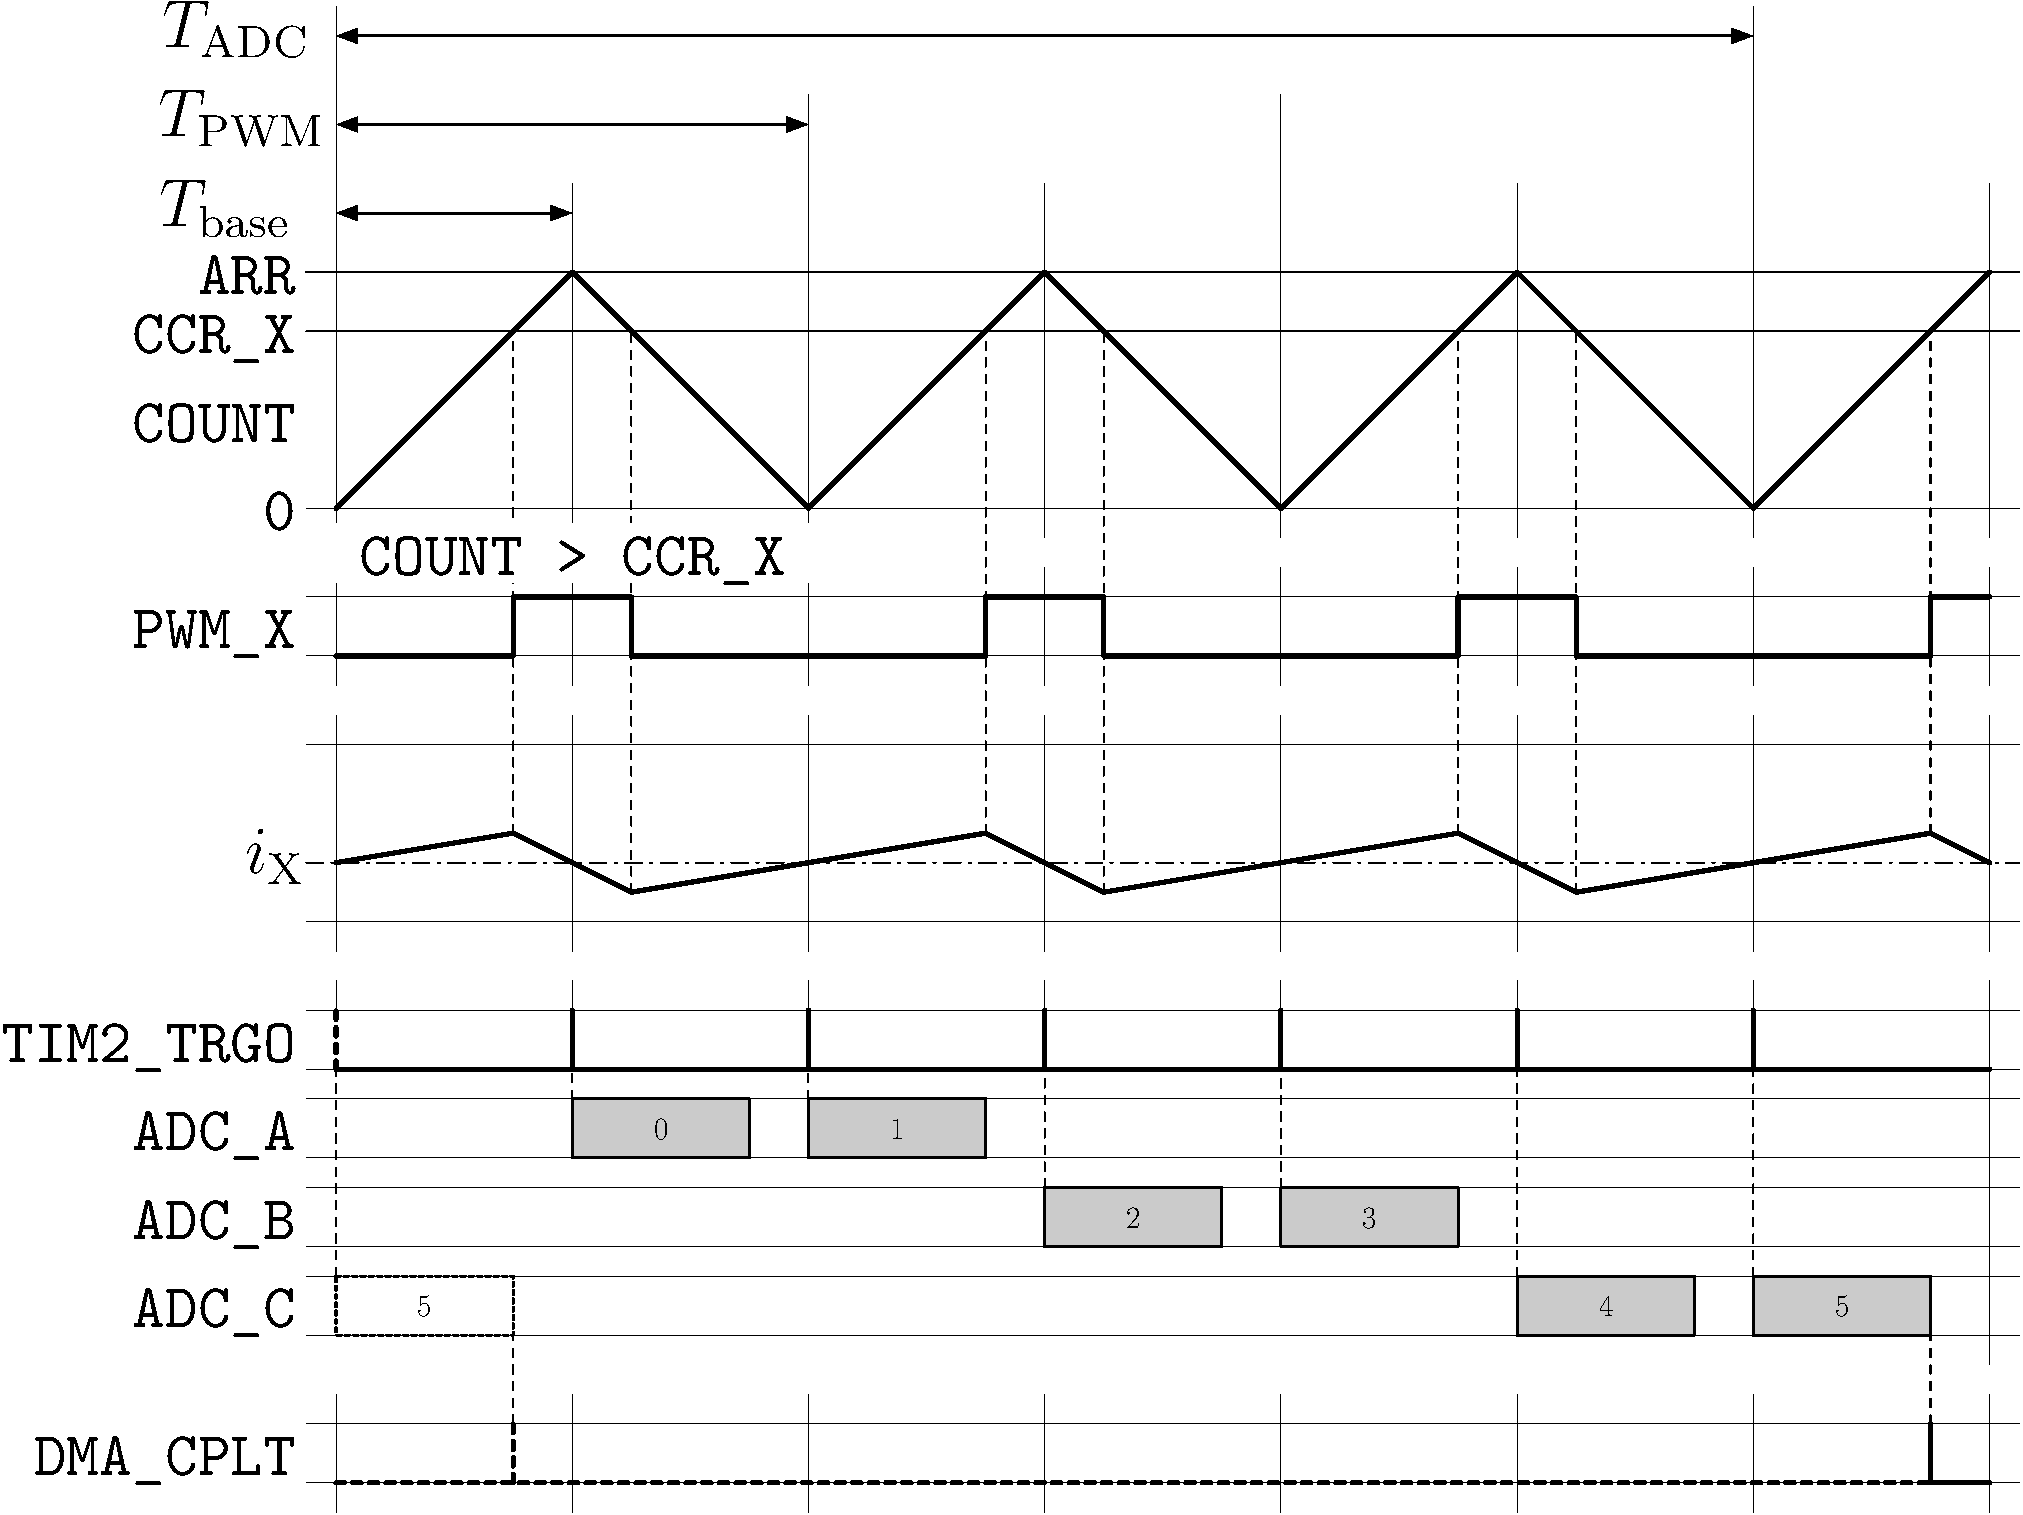
\includegraphics[scale=0.4]{n17-servo-pwm-adc.pdf}
%\caption[PWM and ADC Sync]{Temporal synchronization of PWM output and ADC sampling.}
%\label{fig:pwm-adc}
%\end{center}
%\end{figure}

\subsubsection{ADC Triggering}

As the ADC sampling takes a finite time, it will not quite sample on-center. \texttt{TIM15} is setup to offset by $T_{\textrm{base}} - T_{\textrm{ssaa}}/2$.\footnote{$\unit{6.47}{\micro\second}$ or 1100 CPU cycles for 1700 cycle period.}

\begin{figure}[htbp]
\begin{center}
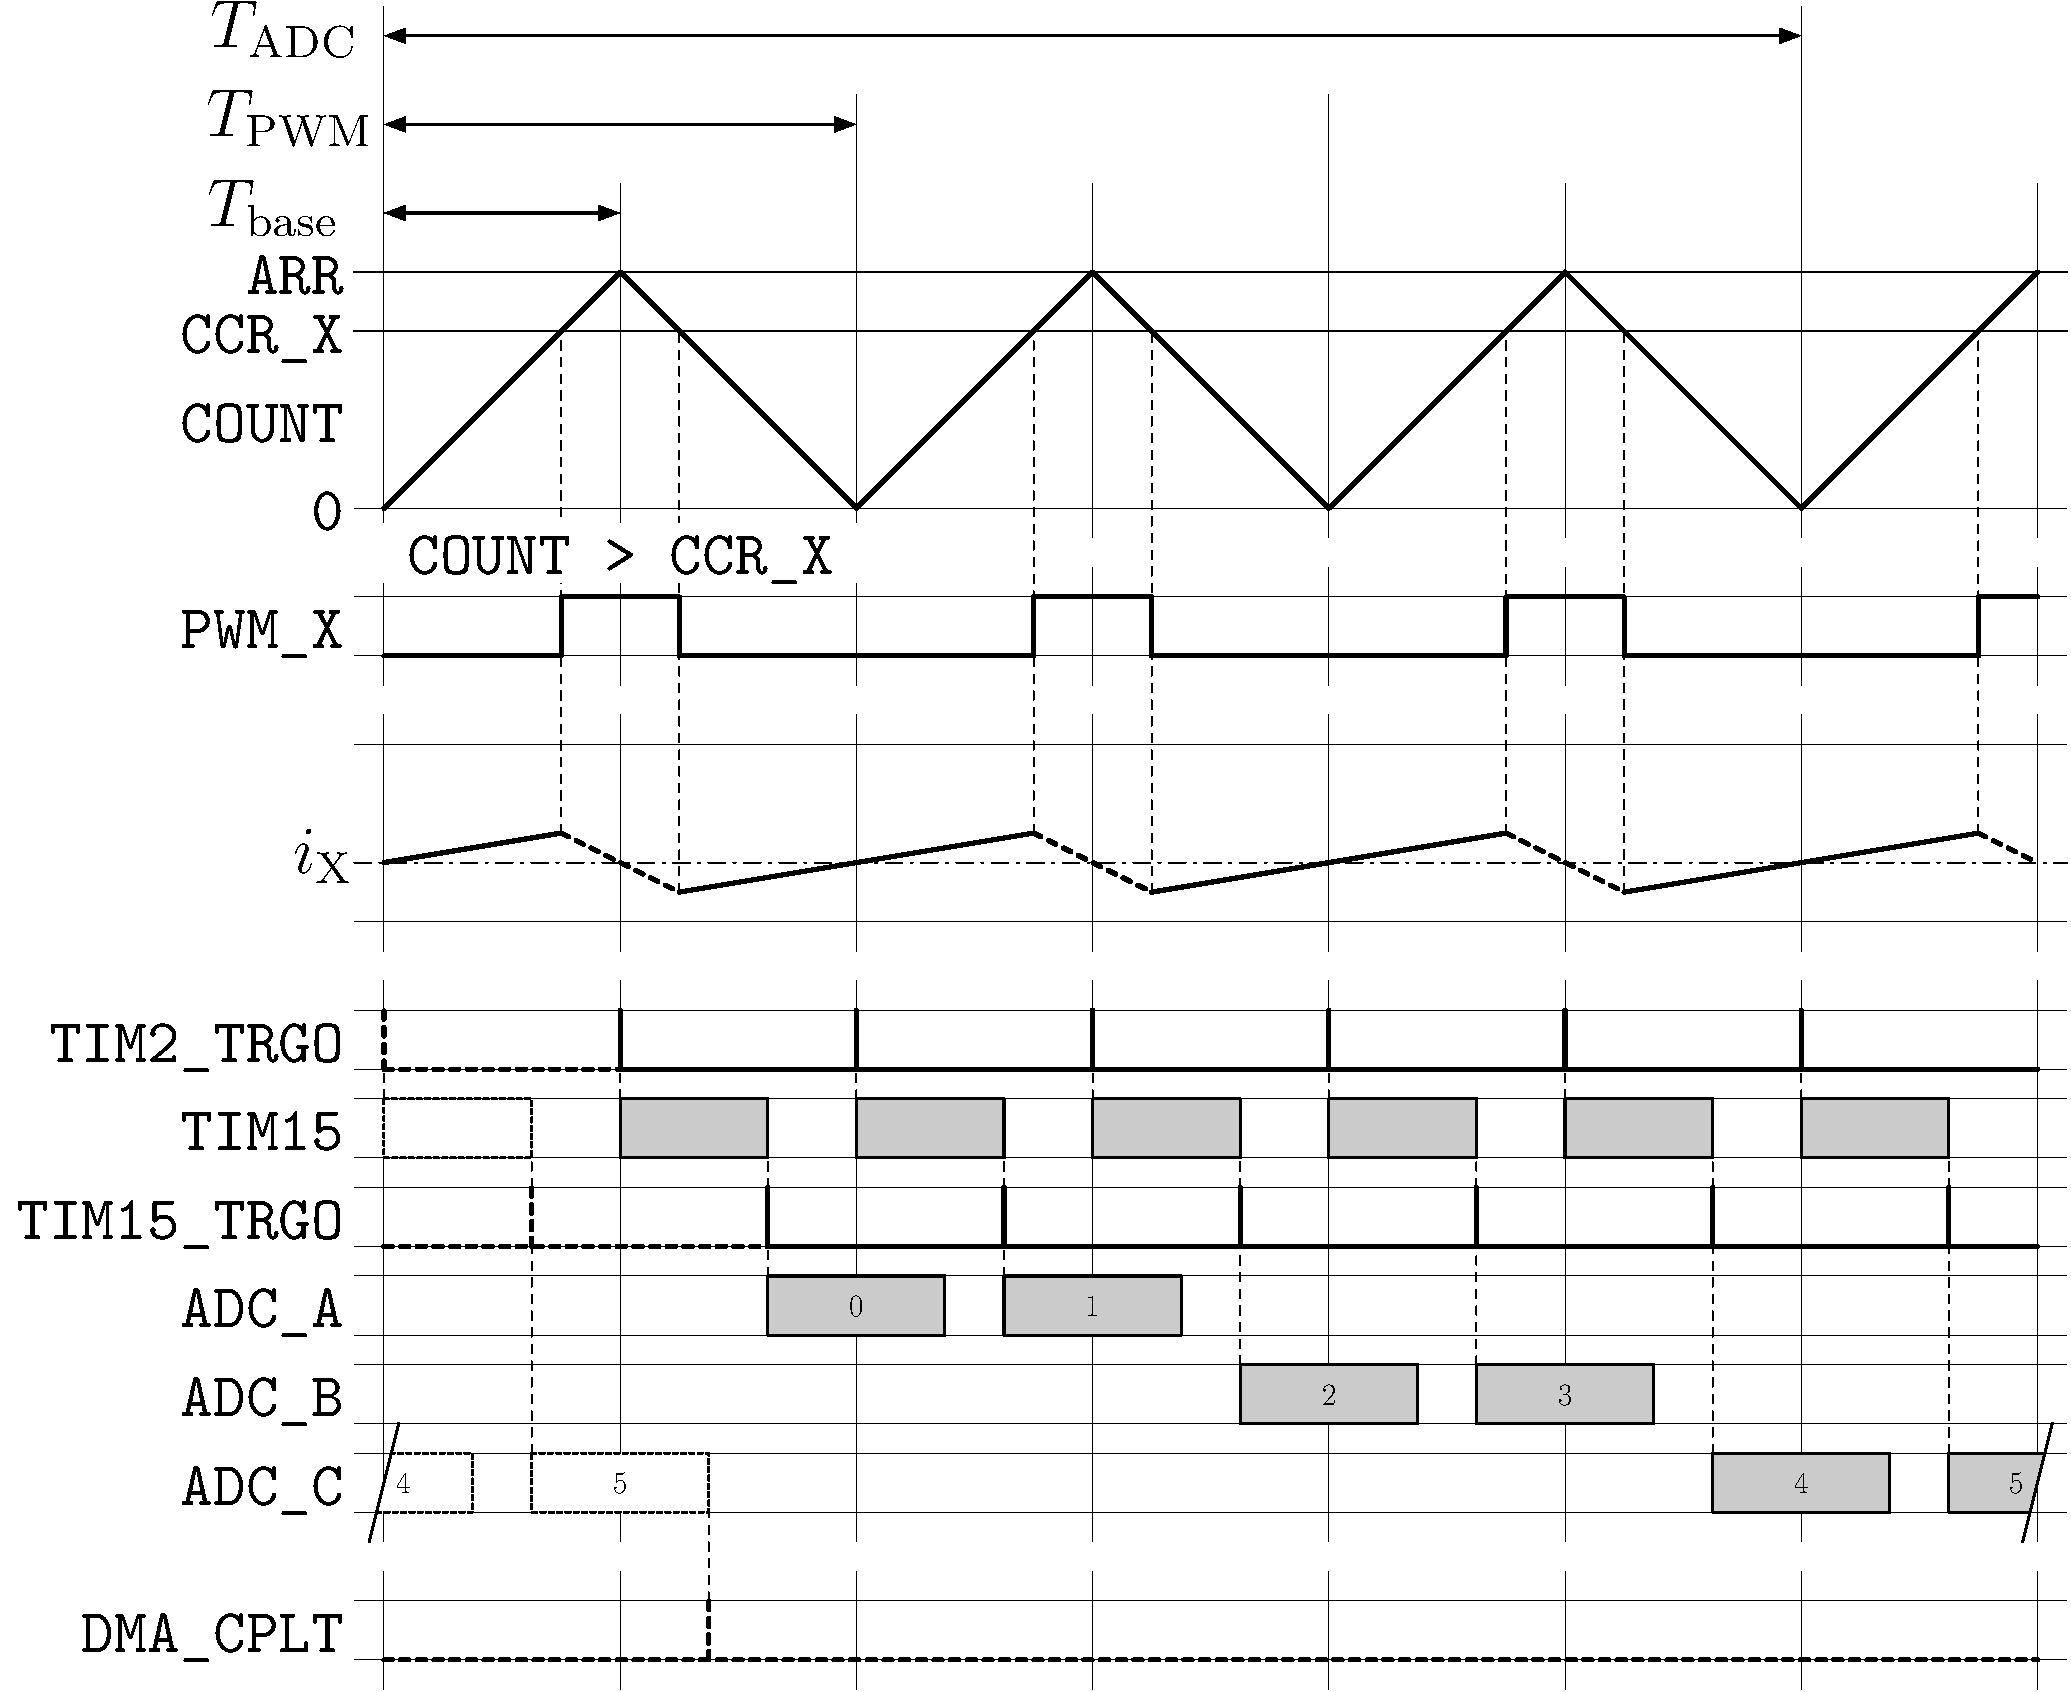
\includegraphics[scale=0.4]{n17-servo-pwm-adc-offset.pdf}
\caption[PWM and ADC Sync with Offset]{Temporal synchronization of PWM output and ADC sampling with centering offset. Adding a triggered timer  (\texttt{TIM15}) as a delay allows offsetting the ADC sampling to occur centered on PWM phases.}
\label{fig:pwm-adc-offset}
\end{center}
\end{figure}

\subsection{Sense Resistor Choice}

The \em DRV8323 \em has a programmable gain between 5 and 40, with 20 being the default. 1206-size resistors can dissipate \unit{1}{\watt}\footnote{\unit{2-3}{\watt} according to datasheets for different resistors, so this is with adequate margin}. For \unit{8}{\ampere}, $P = \unit{0.96}{\watt}$ with $R=\unit{15}{\milli\ohm}$. The sense amplifiers can go up to \unit{0.25}{\volt} short of the supply rails, for a \unit{3.3}{\volt} that leaves \unit{\pm 1.4}{\volt}. The sense voltage $U_S \ @ \  \unit{8}{A}=\unit{120}{\milli\volt}$, thus a gain factor of 5 or 10 would cover the expected current range nicely.

The sense resistor could be made be smaller to reduce power dissipation and allow higher curents, at the expense of reduced resolution.

%// 	// default amp gain factor is G = 20 (5/10/20/40) are available
%// 	// current sense shunts are Rs = 15mOhm
%// 	// sense amp output is centered on VREF/2, max. 0.25V away from rail
%// 	// thus +- 1.4V usable range
%// 	// for 12V operation, 10A would give 150mV, factor of 10 gives full range for 8A
%// 	// return Rs * G


\section{PWM}

The PWM output has to be synchronized with sampling the current sense values. This is done through builtin hardware trigger mechanisms between the different peripherals on the MCU which allow precise timing without CPU involvement.

ADC sampling should happen in the middle of the PWM high/low periods, and to achieve this PWM is run in up/down counting mode, and the ADC readout is triggered at the end of each period.

The PWM base period $T_{\textrm{base}} = \unit{10}{\micro\second}$ ($f_{\textrm{base}} = \unit{100}{\kilo\hertz}$) results in an effective output period of $T_{\textrm{gate}} = \unit{20}{\micro\second}$ ($f_{\textrm{gate}} = \unit{50}{\kilo\hertz}$), and ADC sampling of each channel every $T_{\textrm{sense}} = \unit{60}{\micro\second}$ ($f_{\textrm{sense}} = \unit{16.7}{\kilo\hertz}$). \unit{16.7}{\kilo\hertz} leaves \unit{10.2}{\kilo} instruction cycles per control loop iteration.\footnote{The base frequency could be increased to \unit{120}{\kilo\hertz}, to get $f_{\textrm{ctrl}} = \unit{20}{\kilo\hertz}$. Increasing the PWM frequency does reduce the effective resolution, and reduces the number of available instruction cycles (\unit{8.5}{\kilo} @ \unit{20}{\kilo\hertz}).}

\texttt{TIM2} is setup for driving the gate driver and brake resistor PWM.

\section {ADC}

\subsubsection{ADC Sampling}

\texttt{ADC2} is setup to sample with 12.5 cycles sample time, with 16x oversampling. $f_{\textrm{ADC}} = \unit{170/3}{\mega\hertz}$, and a single channel takes $12.5+12.5$ cycles per sample\footnote{sampling plus conversion}, with $T_{\textrm{sample}} = \unit{0.44}{\micro\second}$. That ends up being $T_{\textrm{ssaa}} = \unit{7.06}{\micro\second}$ with 16x oversampling.


\begin{figure}[htbp]
\begin{center}
\begin{circuitikz} 
\ctikzset{diodes/scale=0.7}
% voltage source
\draw
  (3,-1) -- ++(-3,0) to[european voltage source, v=$U_{\textrm{bus}}$] (0,4) to ++(3,0)
  ;
% diodes
\draw
  (3,0) -- ++(0,0.25)  -- ++(-0.5,0) to[D,l=lo] ++(0,1.5) -- ++(0.5,0) to[short, -*] ++(0.0,0.25)
  -- ++(0,0.25) -- ++(-0.5,0) to[D,l=hi] ++(0,1.5) -- ++(0.5,0) -- ++(0,0.25)
  ;
% switches
\draw
  (3.0,0.25) to[short,*-] ++(0.5,0)
  to[normal open switch] ++(0,1.5) to[short, -*] ++(-0.5,0)
;
\draw
  (3,2.25) to[short,*-] ++(0.5,0)
  to[closing switch] ++(0,1.5) to[short, -*] ++(-0.5,0)
;
% sense resistor
\draw
  (3,-1) to[R,resistors/scale=0.5,l=$R_{\textrm{sense}}$] ++(0,1)
;
% output node
\draw
  (3,2.0) to[short,-o] node[right]{$U=U_{\textrm{bus}}$}(4.0,2.0)
;
\end{circuitikz}
\caption[RL Circuit]{Simplified half-bridge with body diodes and current sense resistor, high-side switch closed.}
\label{fig:halfbridge-diodes}
\end{center}
\end{figure}

\Cref{fig:halfbridge-diodes} illustrates why current cannot flow through $R_{\textrm{sense}}$ when the high-side switch is closed: closing the switch shorts $U$ to $U_{\textrm{bus}}$, thus precluding any current from flowing through the low-side body diode.

With super-sampling, the lack of current flow through the sense resistor while the high-side switch is on must be accounted for. 


\subsubsection{Sampling High-Impedance Sources}

High-impedance voltage dividers will be affected by ADC input impedance. Longest possible sampling times and additional buffer capacitors at the input are advised.

\section{AS5047D Magnetic Encoder on Shaft}

The AS5047D is optionally located in the center of the board, for a direct on-axis configuration. It is a 14-bit magnetic encoder. We use it via its SPI interface. The SPI angle data is updated at \unit{4}{\mega\hertz}.

Propagation delay of sensor is spec'd at \unit{100}{\micro\second} $\pm\unit{10}{\micro\second}$ from sensing to read via SPI. At \unit{8}{\mega\hertz}, SPI read of 16bits takes \unit{2}{\micro\second} nominally, so $\approx\unit{10}{\micro\second}$ for the 4x16bit words seems a reasonable assumption.

The AS5047 clocks out a response at the NEXT 16bit transfer. NSS needs to be asserted during each transfer. SPI $\texttt{CPOL}=0$, and $\texttt{CPHA}=1$, eg. clock is default low, and data is sampled on the falling edge. Unfortunately the STM32G4 SPI peripheral is incapable of asserting NSS via hardware. 

During regular operation, the angle reads can be pipelined, and should be timed to match PWM output and ADC readings. Operating at a \unit{50}{\kilo\hertz} PWM rate means a \unit{20}{\micro\second} period. 


\subsection{AS5047D Readout}

The AS5047D is read out via SPI. It is specified at a \unit{250}{\nano\second} refresh rate at SPI (\unit{4}{\mega\hertz}), with a \unit{90-110}{\micro\second} measurement delay. 

During normal operation, the encoder would be read out once per control cycle. A BLDC may rotate at up to 4000rpm, which is ~67rev/sec, or 419rad/sec. At 20kHz, that's about 9 degrees of rotation.

\subsubsection{Hardware timed SPI reads}

Unfortunately, a native hardware NSS trigger isn't quite possible, but a timer should still be able to trigger the NSS GPIO pin, and then kick off the SPI transfer. The \texttt{TIM2\_TRGO} signal from the \texttt{TIM2\_UP} event is used to center ADC reads, and could also be used to trigger the SPI reads.

The STM32G4 does not have the capability to trigger multiple DMA transfers from the same event, but events can be chained.

\begin{enumerate}
\item Assert encoder NSS (active low)
    \begin{enumerate}
    \item start counter and DMA transfer to GPIO bit clear register
    \item start counter \texttt{TIM8\_CH1}
    \item in one-pulse mode, count a few cycles (AS5047D requires \unit{350}{\nano\second} hold time before clocking, approx. 60 cycles @ \unit{170}{\mega\hertz}) until \texttt{TIM8\_CH1}
    \end{enumerate}
\item Clock out 16bits, read/write
    \begin{enumerate}
    \item start DMA data transfer on \texttt{TIM8\_CH1} (eg. after the timer counted long enough to have the chip select asserted)
    \end{enumerate}
\item Deassert NSS
    \begin{itemize}
    \item Either use \texttt{SPI2\_TX} DMA request as chained source for \texttt{DMA\_GENERATOR0}, which will set the NSS line high again.
    \item Or set NSS high from TX complete interrupt, as exact timing is uncritical, as long as it happens before the next \texttt{TIM2\_UP} event.
    \end{itemize}
\end{enumerate}

\begin{figure}[htbp]
\begin{center}
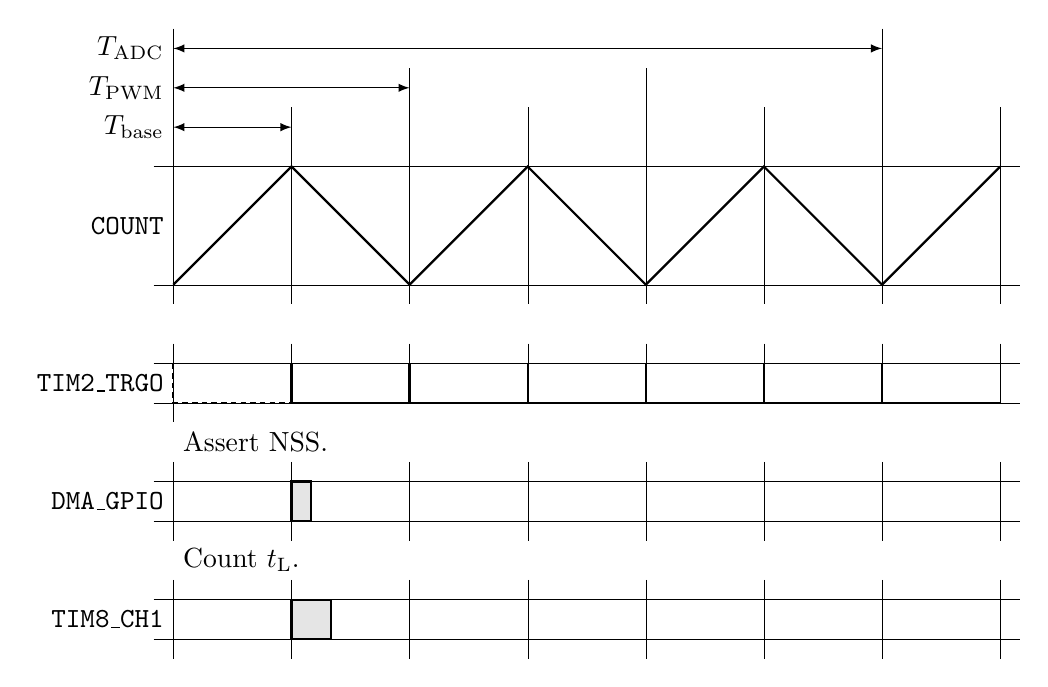
\begin{tikzpicture}[>=latex]
%    \draw (0,0) circle (3);
% times
	\draw[-,ultra thin] (0.0,1.25) -- ++(0,-3.5);
	\draw[<->] (0,1.0) node[anchor=east] {$T_{\textrm{ADC}}$} -- ++(9.0,0);
	\draw[-,ultra thin] (9.0,1.25) -- ++(0,-3.5);
	\draw[<->] (0,0.5) node[anchor=east] {$T_{\textrm{PWM}}$} -- ++(3.0,0);
	\draw[-,ultra thin] (3.0,0.75) -- ++(0,-3.0);
	\draw[-,ultra thin] (6.0,0.75) -- ++(0,-3.0);
	\draw[<->] (0,0.0) node[anchor=east] {$T_{\textrm{base}}$} -- ++(1.5,0);
	\draw[-,ultra thin] (1.5,0.25) -- ++(0,-2.5);
	\draw[-,ultra thin] (4.5,0.25) -- ++(0,-2.5);
	\draw[-,ultra thin] (7.5,0.25) -- ++(0,-2.5);
	\draw[-,ultra thin] (10.5,0.25) -- ++(0,-2.5);
	
	% pwm counter
	\draw[-,ultra thin] (-0.25,-2.0) -- ++(11,0);
	\draw[-,ultra thin] (-0.25,-0.5) -- ++(11,0);
	\draw[-,thick] (0,-2.0) -- ++(1.5,1.5) -- ++(1.5,-1.5) -- ++(1.5,1.5) -- ++(1.5,-1.5) -- ++(1.5,1.5) -- ++(1.5,-1.5) -- ++(1.5,1.5);
	\draw[] (0.0,-1.25) node[anchor=east] {$\texttt{COUNT}$};

	% TIM2
	\node (TIM2) at (0,-3.5) {};
	
  	\draw[-,ultra thin] ($(TIM2) + (0,0.75)$) -- ++(0,-1.0);
	\foreach \x in {1,...,7} 
  		\draw[-,ultra thin] ($(TIM2) + (1.5*\x,0.75)$) -- ++(0,-0.75);
	\draw[-,ultra thin] (-0.25,-3.0) -- ++(11,0);
	\draw[-,ultra thin] (-0.25,-3.5) -- ++(11,0);
	\draw[] (0.0,-3.25) node[anchor=east] {$\texttt{TIM2\_TRGO}$};
	\draw[-,thick,dash pattern=on 2pt off 1.5pt] (0,-3.0) -- ++(0,-0.5) -- ++(1.5,0);
	\foreach\x in {1,...,6} 
  		\draw[-,thick] (1.5*\x,-3.0) -- ++(0,-0.5) -- ++(1.5,0);

	% DMA GPIO
	\node (DMA_GPIO) at (0,-5.0) {};
	\draw ($(DMA_GPIO) + (0.0, 1.0)$) node[anchor=west] {Assert NSS.};
	\foreach \x in {0,...,7} 
  		\draw[-,ultra thin] ($(DMA_GPIO) + (1.5*\x,0.75)$) -- ++(0,-1.0);
	\draw[-,ultra thin] ($(DMA_GPIO) + (-0.25,0.0)$) -- ++(11,0);
	\draw[-,ultra thin] ($(DMA_GPIO) + (-0.25,0.5)$) -- ++(11,0);
	\draw[] ($(DMA_GPIO) + (0,0.25)$) node[anchor=east] {$\texttt{DMA\_GPIO}$};
	\filldraw[thick,fill=black!10!white,draw=black] ($(DMA_GPIO) + (1.5,0.5)$) rectangle ++(0.25,-0.5);

	% TIM8
	\node (TIM8) at (0,-6.5) {};
	\draw ($(TIM8) + (0.0, 1.0)$) node[anchor=west] {Count $t_{\textrm{L}}$.};
	\foreach \x in {0,...,7} 
  		\draw[-,ultra thin] ($(TIM8) + (1.5*\x,0.75)$) -- ++(0,-1.0);
	\draw[-,ultra thin] ($(TIM8) + (-0.25,0.0)$) -- ++(11,0);
	\draw[-,ultra thin] ($(TIM8) + (-0.25,0.5)$) -- ++(11,0);
	\draw[] ($(TIM8) + (0,0.25)$) node[anchor=east] {$\texttt{TIM8\_CH1}$};
	\filldraw[thick,fill=black!10!white,draw=black] ($(TIM8) + (1.5,0.5)$) rectangle ++(0.5,-0.5);

%   	\draw[->,dotted] (-3,0) -- (3,0); % node[anchor=west] {re};
%   	\draw[->,dotted] (0,-3) -- (0,3); % node[anchor=south] {im};
%   	\draw[->] (0,0) -- (30:3) node[anchor=210] {d};
%   	\draw[->] (0,0) -- (120:3) node[anchor=300] {q};
%    \draw[->]  (0:2.7)  node[anchor=315]{$\theta$} arc (0:30:2.7);
%    \draw[->, thick,dashed]  (0,0) -- (30:2.5) node[anchor=300] {$E$};
%    \draw[->, thick,dashed]  (0,0) -- (120:2.5) node[anchor=210] {$\tau$};
%    \draw[->, very thick]  
%        (30:0.5) coordinate (D)
%        (120:1.5) coordinate (Q)
%    	(0,0) -- (D) node[anchor=300] {$i_d$}
%    	(0,0) -- (Q) node[anchor=210] {$i_q$}
%    	(0,0) -- ($(D) + (Q)$) node[anchor=south] {$i$}
%	;
%    \draw[->, very thick]  (0,0) -- (30:0.75) node[anchor=south] {$I_d$};
%    \draw[->, very thick]  (0,0) -- (120:2) node[anchor=0] {$I_q$};
%    \draw[->, very thick]  (0,0) -- ($(30:0.75) + (120:2)$) node[anchor=south] {$I$};
%    \draw[-, dotted]  (30:0.75) -- ($(30:0.75) + (120:2)$) -- (120:2);

\end{tikzpicture}
\caption[AS5047D SPI]{SPI readouts.}
\label{fig:as5047d-spi}
\end{center}
\end{figure}


\section{The RL-Circuit}

\begin{figure}[htbp]
\begin{center}
\begin{circuitikz} \draw
(0,0) to[european voltage source, v=U] (0,4) -- (4,4)
  to[L,l=L,i=i] (4,2)
  to[R,l=R] (4,0) -- (0,0)
;
\end{circuitikz}
\caption[RL Circuit]{RL Circuit Diagram}
\label{fig:RL}
\end{center}
\end{figure}


The governing equation of an RL Series Circuit is 
\begin{align}
\frac{\ud}{\ud t} i &= \frac{U - R i}{L} \\
\frac{\ud^2}{\ud t^2} i &= -\frac{R}{L} \frac{\ud}{\ud t} i
\end{align}
%which can be combined to form
%\begin{align}
%-\frac{L}{R} \frac{\ud^2}{\ud t^2} i &= \frac{U - R i}{L}
%\end{align}
%and simplified to
%\begin{align}
%-\frac{L^2}{R^2} \frac{\ud^2}{\ud t^2} i &= \frac{U}{R} - i\\
%L^2 \frac{\ud^2}{\ud t^2} i &= iR^2 - UR
%\end{align}

\subsubsection{Time Domain}

\begin{align}
i R&= U \left( 1 - e^{-t\frac{R}{L}} \right)
\end{align}


\begin{align}
i &= \frac{U}{R} \left( 1 - e^{-t\frac{R}{L}} \right) \\
\frac{\ud}{\ud t} \imath &= \frac{U}{L} e^{-t\frac{R}{L}} \\
\frac{\ud^2}{\ud t^2} \imath &= -\frac{UR}{L^2} e^{-t\frac{R}{L}}
\end{align}

Logarithmic linear regression of first/second derivative?
\begin{align}
\log \left(\frac{L}{U} \frac{\ud}{\ud t} \imath \right) &= -t\frac{R}{L} \\
\log \left( L \right) - \log \left(U \right) + \log \left(\frac{\ud}{\ud t} \imath \right) &= -t\frac{R}{L} \\
\frac{\ud^2}{\ud t^2} \imath &= -\frac{UR}{L^2} e^{-t\frac{R}{L}}
\end{align}



\subsubsection{Combining for L}

Rearranging both equations to be able to drop $R$
\begin{align}
\frac{R}{L} &= \frac{\frac{U}{L} - \dot{\imath}}{\imath} \\
\frac{R}{L} &= - \frac{ \ddot{\imath}}{ \dot{\imath}}
\end{align}
and combining
\begin{align}
\frac{\frac{U}{L} -  \dot{\imath}}{\imath} &= - \frac{\ddot{\imath}}{ \dot{\imath}} \\
\frac{U}{L} -  \dot{\imath} &= - \frac{\ddot{\imath}}{\dot{\imath}} \imath \\
\frac{U}{L}  \dot{\imath} - \dot{\imath}^2 &= - \ddot{\imath} \imath \\
\frac{U}{L}  \dot{\imath} &= \dot{\imath}^2 - \ddot{\imath} \imath \\
L &= U \frac{ \dot{\imath}}{ \dot{\imath}^2 - \ddot{\imath} \imath}
\end{align}

\subsubsection{Combining for R}
\begin{align}
- R \frac{\dot{\imath}}{\ddot{\imath}} &= U \frac{ \dot{\imath}}{ \dot{\imath}^2 - \ddot{\imath} \imath} \\
- R &= U \frac{ \ddot{\imath}}{ \dot{\imath}^2 - \ddot{\imath} \imath}
\end{align}

\subsubsection{Time Constant}

The above formulas for $R$ and $L$ show that the only difference is the appearance of the first vs. second differential of the current in the nominator. As the current curve is an exponential function, both differentials have the same shape, but differ in magnitude by $\tau=L/R$, and thus 
\begin{align}
\tau &= - \frac{\dot{\imath}}{\ddot{\imath}}
\end{align}

\subsection{R Estimation}

The resistance of the circuit can be easily estimated by applying some low PWM duty cycle long enough to reach steady state, and measuring the current.
\begin{align}
R &= D\frac{U}{\imath}
\end{align}

\subsection{L Estimation with a Known R}

Reformulating
\begin{align}
\frac{\ud}{\ud t} i &= \frac{U - R i}{L}
\end{align}
into
\begin{align}
L &= \frac{U - R i}{\frac{\ud}{\ud t} i}
\end{align}
allows inductance estimation with a relatively simple formula.

\subsection{Impedance Estimation}

Exciting a motor coil with a sinusoidal voltage, and measuring the resulting current phase difference and amplitude, the impedance and thus inductance can be calculated. Assuming a pure sinusoidal signal without harmonics,
\begin{gather}
\begin{aligned}
|Z| &= \frac{U_{\textrm{RMS}}}{i_{\textrm{RMS}}} \\
Z &= R + j X \\
Z &= |Z| \left(\cos \theta + j \sin \theta \right)
\end{aligned}
\end{gather}

\subsubsection{Inductance from Impedance}

\begin{gather}
\begin{aligned}
X &= \sqrt{|Z|^2 - R^2} \\
X_L &= \omega L
\end{aligned}
\end{gather}

It looks like this method yields more accurate results than anything looking at $\frac{\ud}{\ud t} i$. This is not surprising: noise and offsets can be removed more effectively as $L$ is computed from averaged current readings, vs.\ being computed from each individual current reading and then averaged.

This method still seems to over-estimate inductance, but seems to get significantly closer. Interestingly, for a 2-phase motor, the estimated impedance running through both phases gets closer to the specified values than both individual phase measurements.

\subsubsection{Phase Estimation}

The phase angle $\theta$ between $U=U_{\textrm{peak}}\sin \omega$ and $i=i_{\textrm{peak}}\sin \left(\omega+\theta\right)$ can be found as the DC component of the composite signal $U(\omega) \times i(\omega)$:
\begin{gather}
\begin{aligned}
U(\omega) \times i(\omega) &= \frac{\cos \theta - \cos\left(2\omega+\theta\right)}{2} \\
\overline{U \times i} &= \frac{1}{2\pi}\int_0^{2\pi} U \times i \ud \omega = U_{\textrm{peak}} i_{\textrm{peak}}\frac{\cos \theta}{2} \\
\cos \theta &= 2 \frac{\overline{U \times i}}{U_{\textrm{peak}} i_{\textrm{peak}}} =\frac{\overline{U \times i}}{U_{\textrm{RMS}} i_{\textrm{RMS}}}
\end{aligned}
\end{gather}

\subsubsection{Resistance from Impedance and Phase}

\begin{gather}
\begin{aligned}
R &= |Z| \cos \theta = \frac{\overline{U i}}{i_{\textrm{RMS}}^2}
\end{aligned}
\end{gather}

As resistance depends on $R \approx \cos \theta$, it is very sensitive to phase shifts, and thus not very reliable for estimation


\subsection{Simultaneous LR Estimation}

Sampling a  applied voltage $U$ step function at fixed intervals $T$, for samples $i_0, i_1, \ldots, i_n$ with t $t>0,n=t/T$, we can compute the differentiations in different ways.

\subsubsection{N3 Sampling}

Assuming linearity around $n=1$:
\begin{align}
{\imath} &= \frac{1}{3} (\imath_0 + \imath_1 + \imath_2) \\
\dot{\imath} &= \frac{1}{2T} (\imath_2 - \imath_0) \\
\ddot{\imath} &= \frac{1}{T^2} (\imath_2 - 2\imath_1 + \imath_0)
\end{align}
and
\begin{align}
L &= U \frac{\dot{\imath}}{\dot{\imath}^2 - \ddot{\imath} \imath}
\end{align}


\section{Single Phase Analysis}

\subsection{Motor Phase Model}

\begin{figure}[htbp]
\begin{center}
\begin{subfigure}[t]{0.45\textwidth}
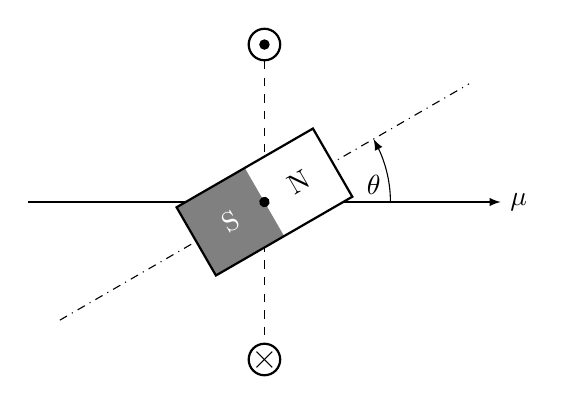
\begin{tikzpicture}[>=latex]
    % flux axis
    \draw[-,dashed] (0,2) -- (0,-2);
  	\draw[->] (-3,0) -- (3,0) node[anchor=west] {$\mathbf{\mu}$};
	% out winding
    \filldraw[fill=white,thick] (0,2) circle (0.2);
    \fill (0,2) circle (0.0667);
    % in winding
    \filldraw[fill=white,thick] (0,-2) circle (0.2);
    \draw (0.1,-2.1) -- ++(-0.2, 0.2);
    \draw (-0.1,-2.1) -- ++(0.2, 0.2);
	% magnet
	\begin{scope}[rotate=30]
    	\draw[-,dashdotted] (-3,0) -- (3,0);
  		\fill[fill=white] (-1,-0.5) rectangle ++(2,1);
  		\fill[fill=gray] (-1,-0.5) rectangle ++(1,1);
  		\draw[-,thick] (-1,-0.5) rectangle ++(2,1);
   		\draw[] (-0.5,0) node[rotate=30,text=white]{S};
   		\draw[] (0.5,0) node[rotate=30]{N};
   		\fill (0,0) circle (0.0667);
	\end{scope}
	% rotation
    \draw[->]  (0:1.6)  node[anchor=315]{$\theta$} arc (0:30:1.6);

\end{tikzpicture}
\caption{single phase winding and rotor magnet}
\end{subfigure}
\hspace*{\fill}
\begin{subfigure}[t]{0.45\textwidth}
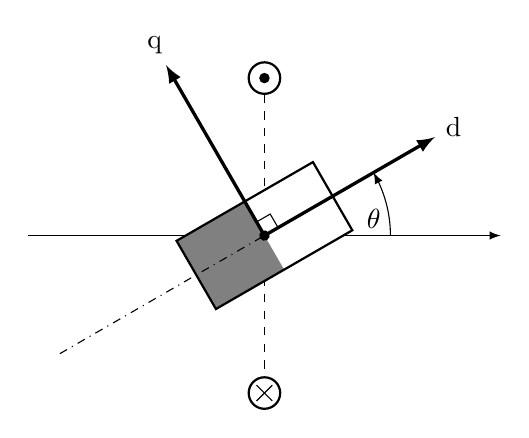
\begin{tikzpicture}[>=latex]
    % flux axis
    \draw[-,dashed] (0,2) -- (0,-2);
   	\draw[->] (-3,0) -- (3,0);
	% out winding
    \filldraw[fill=white,thick] (0,2) circle (0.2);
    \fill (0,2) circle (0.0667);
%    \filldraw[fill=lightgray,thick] (-2,0) circle (0.2);
%    \fill (-2,0) circle (0.0667);
    % in winding
    \filldraw[fill=white,thick] (0,-2) circle (0.2);
    \draw (0.1,-2.1) -- ++(-0.2, 0.2);
    \draw (-0.1,-2.1) -- ++(0.2, 0.2);
%    \filldraw[fill=lightgray,thick] (2,0) circle (0.2);
%    \draw (2.1,-0.1) -- ++(-0.2, 0.2);
%    \draw (1.9,-0.1) -- ++(0.2, 0.2);
	% magnet
	\begin{scope}[rotate=30]
  		\fill[fill=white] (-1,-0.5) rectangle ++(2,1);
  		\fill[fill=gray] (-1,-0.5) rectangle ++(1,1);
  		\draw[-,thick] (-1,-0.5) rectangle ++(2,1);
%   		\draw[] (-0.5,0) node[rotate=30,text=white]{S};
%   		\draw[] (0.5,0) node[rotate=30]{N};
    	\draw[-,dashdotted] (-3,0) -- (0,0);
   		\draw[->, very thick] (0,0) -- (2.5,0) node[anchor=210]{d};
   		\draw[->, very thick] (0,0) -- (0,2.5) node[anchor=300]{q};
   		\draw[-] (0,0.2) -- (0.2,0.2) -- (0.2,0);
   		\fill (0,0) circle (0.0667);
	\end{scope}
	% rotation
    \draw[->]  (0:1.6)  node[anchor=315]{$\theta$} arc (0:30:1.6);

\end{tikzpicture}
\caption{QD coordinates}
\end{subfigure}

\caption[Motor Phase Model]{Single phase winding model. The rotor magnet is at angle $\theta$ relative to the winding's principal field axis $\mu$. The QD coordinate system is aligned with the rotor's magnetic field, instead of the winding's. The \em direct \em component is aligned with the rotor magnet poles, and the \em quadrature \em component is perpendicular to them, electrically.}
\label{fig:singlephaseqd}
\end{center}
\end{figure}

\begin{figure}[htbp]
\begin{center}
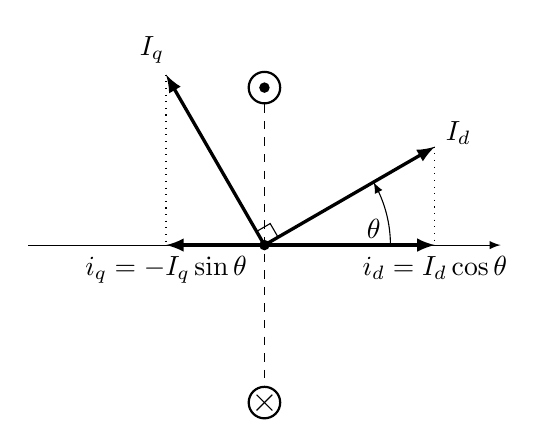
\begin{tikzpicture}[>=latex]
    % flux axis
    \draw[-,dashed] (0,2) -- (0,-2);
   	\draw[->] (-3,0) -- (3,0); % node[anchor=south west] {$\mathbf{\mu}$};
	% out winding
    \filldraw[fill=white,thick] (0,2) circle (0.2);
    \fill (0,2) circle (0.0667);
    % in winding
    \filldraw[fill=white,thick] (0,-2) circle (0.2);
    \draw (0.1,-2.1) -- ++(-0.2, 0.2);
    \draw (-0.1,-2.1) -- ++(0.2, 0.2);
	% magnet
	\begin{scope}[rotate=30]
   		\draw[->,very thick] (0,0) -- (2.5,0) node[anchor=210]{$I_d$};
   		\draw[->,very thick] (0,0) -- (0,2.5) node[anchor=300]{$I_q$};
   		\draw[-] (0,0.2) -- (0.2,0.2) -- (0.2,0);
	\end{scope}
	% rotation
    \draw[->]  (0:1.6)  node[anchor=315]{$\theta$} arc (0:30:1.6);
    % projections
  
    \fill (0,0) circle (0.0667);
    \draw[-,dotted] (120:2.5) -- ( {-2.5*sin(30)}, 0 );
    \draw[->,very thick] (0,0) -- ( {-2.5*sin(30)}, 0 ) node[sloped,below] {$i_q = -I_q \sin \theta$};
    \draw[-,dotted] (30:2.5) -- ( {2.5*cos(30)}, 0 );
    \draw[->,very thick] (0,0) -- ( {2.5*cos(30)}, 0 ) node[sloped,below] {$i_d = I_d \cos \theta$};

\end{tikzpicture}

\caption[QD to Phase Projection]{Projection of the QD coordinate system currents onto the principal axis of a single winding.}
\label{fig:qdproj}
\end{center}
\end{figure}


\begin{figure}[htbp]
\begin{center}
\begin{circuitikz}[]
\draw (0,5) node[anchor=180]{$U$}
  to[V,v<=$E$,i=$i$,o-*] ++(0,-2) node[anchor=180]{$U'$}
  to[L=$L$] ++(0,-1.5)
  to[R=$R$,-] ++(0,-1.5) node[rground]{}
;
\end{circuitikz}
\caption[Single Phase Model]{Single phase motor winding model that is composed of a passive LR part, and the BEMF component $E$.}
\label{fig:singlephase}
\end{center}
\end{figure}

\begin{figure}[htbp]
\begin{center}
\begin{tikzpicture}[>=latex]
%    \draw (0,0) circle (3);
   	\draw[->,dotted] (-3,0) -- (3,0); % node[anchor=west] {re};
   	\draw[->,dotted] (0,-3) -- (0,3); % node[anchor=south] {im};
   	\draw[->] (0,0) -- (30:3) node[anchor=210] {d};
   	\draw[->] (0,0) -- (120:3) node[anchor=300] {q};
    \draw[->]  (0:2.7)  node[anchor=315]{$\theta$} arc (0:30:2.7);
%    \draw[->, thick,dashed]  (0,0) -- (30:2.5) node[anchor=300] {$E$};
%    \draw[->, thick,dashed]  (0,0) -- (120:2.5) node[anchor=210] {$\tau$};
%    \draw[->, very thick]  
%        (30:0.5) coordinate (D)
%        (120:1.5) coordinate (Q)
%    	(0,0) -- (D) node[anchor=300] {$i_d$}
%    	(0,0) -- (Q) node[anchor=210] {$i_q$}
%    	(0,0) -- ($(D) + (Q)$) node[anchor=south] {$i$}
%	;
    \draw[->, very thick]  (0,0) -- (30:0.75) node[anchor=south] {$I_d$};
    \draw[->, very thick]  (0,0) -- (120:2) node[anchor=0] {$I_q$};
    \draw[->, very thick]  (0,0) -- ($(30:0.75) + (120:2)$) node[anchor=south] {$I$};
    \draw[-, dotted]  (30:0.75) -- ($(30:0.75) + (120:2)$) -- (120:2);

\end{tikzpicture}
\caption[Phasors]{Current phasor for a rotating stator field and PM rotor in a QD coordinate system.}
%\label{fig:singlephase}
\end{center}
\end{figure}

The single phase winding electrical model
\begin{gather}
\begin{aligned}
\label{eq:singlephase} 
U &= E + R \imath + L \frac{\partial \imath}{\partial t}
\end{aligned}
\end{gather}
as depicted in \cref{fig:singlephase}, with a sinusoidal BEMF voltage
\begin{gather}
\begin{aligned}
\label{eq:sineemf} 
E_k &= k_e \omega_m \cos \left( n \theta_m + \phi_{0} \right) = k_e \omega_m \cos \left( \theta_{e} + \phi_0 \right)
\end{aligned}
\end{gather}
is the starting point for modeling motor windings for control purposes.

The BEMF component $E$ is only dependent on rotor position and speed, while the impedance component $L \frac{\partial \imath}{\partial t} + R\imath$ is only dependent the current. Under constant-speed and torque conditions, both are in sync with a speed and torque dependent phase shift.

Assuming a sinusoidal magnetic characteristic, the torque contribution from each phase is
\begin{gather}
\begin{aligned}
\tau &= - k \sin \left( \theta_e + \phi_{0}\right) \cdot \imath.
\end{aligned}
\end{gather}

The phase current $\imath$ can be decomposed, as shown in \cref{fig:qdproj}, into a \em direct \em component that is synchronously in-phase with the rotor magnet
\begin{gather}
\begin{aligned}
\imath_d &= I_d \cos \left( \theta_e + \phi_{0}\right) = I_d \cos \left( \theta \right),
\end{aligned}
\end{gather}
and an orthogonal \em quadrature \em component that is in-phase with the torque producing component of the magnetic field
\begin{gather}
\begin{aligned}
\imath_q &= - I_q \sin \left( \theta_e + \phi_{0}\right) = - I_q \sin \left( \theta \right).
\end{aligned}
\end{gather}
The quadrature component $\imath_q$ is strictly contributing to torque, while $\imath_d$ has a net zero effect, and the total current magnitude is described by
\begin{gather}
\begin{aligned}
I^2 &= I_d^2 + I_q^2.
\end{aligned}
\end{gather}

\subsection{Field Oriented Control}

\em Field Oriented Control \em adjusts the winding voltage's phase angle to keep the current phase locked to the motor angle, extracting maximum torque for a given motor current, regardless of motor speed. However, when shifting the current phase, the contributions to the voltage and torque waveforms change, and this can be used for
\begin{itemize}
\item field weakening, to increase top speed at the expense of available torque,
\item and flux braking, to dissipate excess DC bus voltage without changing the output torque.
\end{itemize}

\subsubsection{Full Winding Equation}

The complete motor winding voltage, in terms of QD currents, is thus given by 
\begin{gather}
\begin{aligned}
%\label{eq:singlephase} 
U &= E + R (\imath_d + \imath_q) + L \frac{\partial (\imath_d + \imath_q)}{\partial t} \\
%U &= E + R I_d \cos \left( \theta \right) - R I_q \sin \left( \theta \right) \\
%&\quad - L \omega_e I_d \sin \left( \theta \right) - L \omega_e I_q \cos \left( \theta \right) \\
%&\quad + L \frac{\partial I_d}{\partial t} \cos \left(\theta \right) - L \frac{\partial I_q}{\partial t} \sin \left(\theta \right) \\
&= - ( R I_q + L \omega_e I_d + L \frac{\partial I_q}{\partial t})\sin \left( \theta \right) \\
&\quad + ( k_e \omega_e + R I_d - L \omega_e I_q + L \frac{\partial I_d}{\partial t}) \cos \left( \theta \right)
\end{aligned}
\end{gather}
Thus, the direct and quadrature components of $U$ are   
\begin{gather}
\begin{aligned}
%\label{eq:singlephase} 
U_q &= R I_q + L \omega_e I_d + L \frac{\partial I_q}{\partial t} \\
U_d &= k_e \omega_e + R I_d - L \omega_e I_q + L \frac{\partial I_d}{\partial t}
\end{aligned}
\end{gather}
for a magnitude of 
\begin{gather}
\begin{aligned}
%\label{eq:singlephase} 
U^2 &= U_d^2 + U_q^2 \\
	&= ( R I_q + L \omega I_d + L \frac{\partial I_q}{\partial t})^2 + ( k_e \omega + R I_d - L \omega I_q + L \frac{\partial I_d}{\partial t})^2 \\
%	&= R^2 I_q^2 + L^2 \omega^2 I_d^2 + L^2 \left( \frac{\partial I_q}{\partial t} \right)^2 + 2 R I_q L \omega I_d + 2 L \omega I_d L \frac{\partial I_q}{\partial t} + 2 R I_q L \frac{\partial I_q}{\partial t} \\
%	&\quad + k_e^2 \omega^2 + R^2 I_d^2 + L^2 \omega^2 I_q^2 + L^2 \left(\frac{\partial I_d}{\partial t}\right)^2 \\
%	&\quad + 2 k_e \omega R I_d - 2 k_e \omega L \omega I_q + 2 k_e \omega L \frac{\partial I_d}{\partial t} \\
%	&\quad - 2 R I_d L \omega I_q + 2 R I_d L \frac{\partial I_d}{\partial t} - 2 L \omega I_q L \frac{\partial I_d}{\partial t}\\
	&= \left(R^2 + L^2 \omega^2 \right) I^2 + L^2 \left(\frac{\partial I_d}{\partial t}\right)^2 + L^2 \left(\frac{\partial I_q}{\partial t}\right)^2 + k_e^2 \omega^2\\
%	&\quad - R L \omega I_d I_q + R L \omega I_d I_q
	&\quad + 2 R L \left( I_d \frac{\partial I_d}{\partial t} + I_q \frac{\partial I_q}{\partial t} \right) \\
	&\quad + 2 L^2 \omega \left(I_d \frac{\partial I_q}{\partial t} - I_q \frac{\partial I_d}{\partial t} \right) \\ 
	&\quad + 2 k_e \omega \left(R I_d - L \omega I_q + L \frac{\partial I_d}{\partial t} \right).
\end{aligned}
\end{gather}

\subsubsection{Constant Speed Analysis}

Assuming constant speed and current, the equation simplifies to
\begin{gather}
\begin{aligned}
%\label{eq:singlephase} 
U^2 &= \left(R^2 + L^2 \omega^2 \right) I^2 + k_e^2 \omega^2  + 2 k_e \omega \left( R I_d - L \omega I_q \right),
\end{aligned}
\end{gather}
from which we can see that $\left( R I_d - L \omega I_q \right)$ remains to influence the magnitude of $U$ by varying $I_d, I_q$. The ratio of the two can be varied via the phase angle $\alpha$, relative to maximum torque, with $I_d = - I \sin \alpha$ and $I_q = I \cos \alpha$ without changing the current magnitude $I$. Differentiating 
\begin{gather}
\begin{aligned}
%\label{eq:singlephase} 
R I_d - L \omega_e I_q &= I \left( - R \sin \alpha - L \omega \cos \alpha \right)
\end{aligned}
\end{gather}
with respect to $\alpha$ yields
\begin{gather}
\begin{aligned}
%\label{eq:singlephase} 
\frac{\partial}{\partial \alpha} \left(- R \sin \alpha - L \omega \cos \alpha \right) &= - R \cos \alpha + L \omega \sin \alpha,
\end{aligned}
\end{gather}
which shows that as we move away from $\alpha = 0$, the magnitude of the phase voltage $U$ can be decreased. This happens when
\begin{gather}
\begin{aligned}
%\label{eq:singlephase} 
- R \cos \alpha - L \omega \sin \alpha < 0,
\end{aligned}
\end{gather}
and thus when
\begin{gather}
\begin{aligned}
%\label{eq:singlephase} 
- \frac{R}{L \omega} < \tan \alpha,
\end{aligned}
\end{gather}
changing the current phase $\alpha$ will result in reduced phase voltage.

\section{3-Phase Star}


\begin{figure}[htbp]
\begin{center}
\begin{subfigure}[t]{0.45\textwidth}
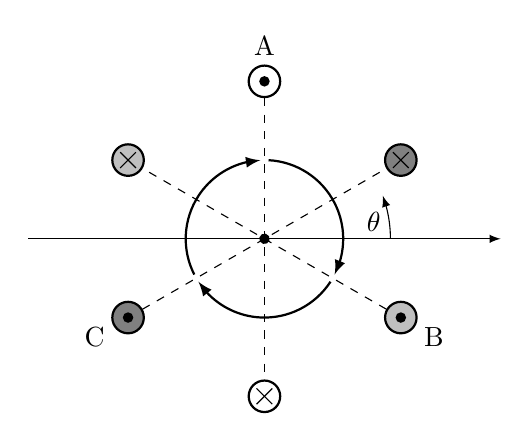
\begin{tikzpicture}[>=latex]
    % flux axis
    \draw[-,dashed] (0,2.2) node[anchor=270]{A};
    \draw[-,dashed] (210:2.2) node[anchor=30]{C};
    \draw[-,dashed] (330:2.2) node[anchor=150]{B};
    \draw[-,dashed] (0,2) -- (0,-2);
    \draw[-,dashed] (210:2.0) -- (30:2);
    \draw[-,dashed] (330:2.0) -- (150:2.0);
   	\draw[->] (-3,0) -- (3,0);
	% out winding
    \filldraw[fill=white,thick] (0,2) circle (0.2);
    \fill (0,2) circle (0.0667);
    \filldraw[fill=gray,thick] (210:2.0) circle (0.2);
    \fill (210:2.0) circle (0.0667);
    \filldraw[fill=lightgray,thick] (330:2.0) circle (0.2);
    \fill (330:2.0) circle (0.0667);
    % in winding
    \filldraw[fill=white,thick] (0,-2) circle (0.2);
    \draw (0.1,-2.1) -- ++(-0.2, 0.2);
    \draw (-0.1,-2.1) -- ++(0.2, 0.2);
    \filldraw[fill=gray,thick] (30:2.0) circle (0.2);
    \draw ($(30:2.0) + (0.1,-0.1)$) -- ++(-0.2, 0.2);
    \draw ($(30:2.0) + (-0.1,-0.1)$) -- ++(0.2, 0.2);
    \filldraw[fill=lightgray,thick] (150:2.0) circle (0.2);
    \draw ($(150:2.0) + (0.1,-0.1)$) -- ++(-0.2, 0.2);
    \draw ($(150:2.0) + (-0.1,-0.1)$) -- ++(0.2, 0.2);
	% magnet
	\begin{scope}[rotate=30]
%  		\fill[fill=white] (-1,-0.5) rectangle ++(2,1);
%  		\fill[fill=gray] (-1,-0.5) rectangle ++(1,1);
%  		\draw[-,thick] (-1,-0.5) rectangle ++(2,1);
%   		\draw[] (-0.5,0) node[rotate=30,text=white]{S};
%   		\draw[] (0.5,0) node[rotate=30]{N};
%    	\draw[-,dashdotted] (-3,0) -- (0,0);
%   		\draw[->, very thick] (0,0) -- (2.5,0) node[anchor=210]{d};
%   		\draw[->, very thick] (0,0) -- (0,2.5) node[anchor=300]{q};
%   		\draw[-] (0,0.2) -- (0.2,0.2) -- (0.2,0);
   		\fill (0,0) circle (0.0667);
	\end{scope}
	% rotation
    \draw[->]  (0:1.6)  node[anchor=315]{$\theta$} arc (0:20:1.6);
    % phase to phase arrows
    \draw[->,thick]  (87:1.0)  arc (87:-27:1.0);
    \draw[->,thick]  (-33:1.0)  arc (-33:-147:1.0);
    \draw[->,thick]  (-153:1.0)  arc (-153:-267:1.0);

\end{tikzpicture}
\caption{Phases}
\end{subfigure}
\hspace*{\fill}
\begin{subfigure}[t]{0.45\textwidth}
\begin{circuitikz}[
	R/.style={european resistor}
]
\draw (0,3) node[anchor=270]{$U$}
  to[R,l=$A$,f=$i_A$,o-] ++(0,-2)
  to[short] ++(0,-1) node[anchor=210]{$N$}
;
\draw (-2.598,-1.5) node[anchor=30]{$V$}
  to[R,l=$B$,f=$i_B$,o-] ++(1.732, 1.0)
  to[short,] ++(0.866, 0.5)
;
\draw (2.598,-1.5) node[anchor=150]{$W$}
  to[R,l=$C$,f=$i_C$,o-] ++(-1.732, 1.0)
  to[short,-*] ++(-0.866, 0.5)
;

\end{circuitikz}
\caption{Star Connection}
\end{subfigure}

\caption[3-Phase Star]{3-Phase Star / Wye Connection. Phases are arranged clockwise (physically \unit{-120}{\degree}) with a resultant $\phi = \unit{120}{\degree}$ electrical offset.}
\label{fig:star}
\end{center}
\end{figure}


\begin{figure}[htbp]
\begin{center}
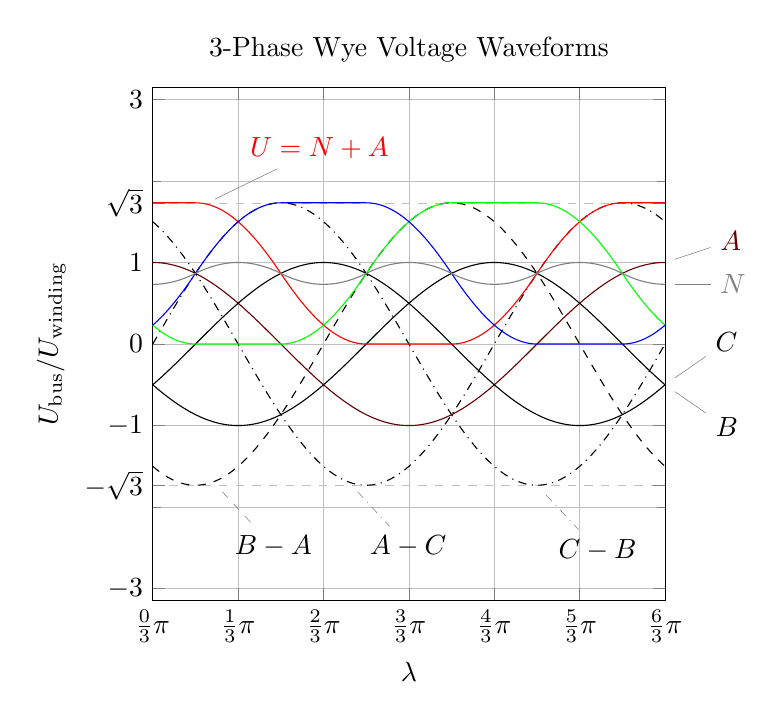
\begin{tikzpicture}[>=latex]
	\begin{axis}[
	width=0.667\textwidth,
	height=0.667\textwidth,
	title=3-Phase Wye Voltage Waveforms, xlabel={$\lambda$}, ylabel={$U_{\mathrm{bus}} / U_{\mathrm{winding}}$}, xmin=0, xmax=2*pi, clip=false,
	axis equal=true,
	enlarge x limits=false,
	xmajorgrids,
	ymajorgrids,
	yminorgrids,
	xtick={0,pi/3, 2*pi/3, pi, 4/3*pi, 5/3*pi, 2*pi},
	xticklabels={{$\frac{0}{3}\pi$}, {$\frac{1}{3}\pi$}, {$\frac{2}{3}\pi$}, {$\frac{3}{3}\pi$}, {$\frac{4}{3}\pi$}, {$\frac{5}{3}\pi$}, {$\frac{6}{3}\pi$}},
	ytick={-3, -sqrt(3), -1, 0, 1, sqrt(3), 3},
	yticklabels={{$-3$}, {$-\sqrt{3}$}, {$-1$}, {$0$}, {$1$}, {$\sqrt{3}$}, {$3$}},
	minor ytick={-3,-2,-1,0,1,2,3},
	major y grid style={dashed,very thin},
	major x grid style={very thin},
	minor y grid style={very thin},
	]
	\addplot[domain=0:2*pi,samples=361,red!40!black] {cos(deg(x))} node [pos=1,pin=3:{$A$}] {};
	\addplot[domain=0:2*pi,samples=361,green!0!black] {cos(deg(x)+120)} node [pos=1,pin=-30:{$B$}] {};
	\addplot[domain=0:2*pi,samples=361,blue!0!black] {cos(deg(x)+240)} node [pos=1,pin=30:{$C$}] {};
	\addplot[domain=0:2*pi,samples=361,dashed] {sqrt(3)*cos(deg(x)+150)} node [pos=1/12,pin=-75:{$B - A$}] {};
	\addplot[domain=0:2*pi,samples=361,dashdotted] {sqrt(3)*cos(deg(x)+270)} node [pos=9/12,pin=-75:{$C - B$}] {};
	\addplot[domain=0:2*pi,samples=361,dashdotted] {sqrt(3)*cos(deg(x)+30)} node [pos=5/12,pin=-75:{$A - C$}] {};
	% "saddle" type driving 
%	\addplot[domain=0:2*pi,samples=361,red] {max(0, max(cos(deg(x)) - cos(deg(x)+120), cos(deg(x)) - cos(deg(x)+240)))} node[pos=1/12,pin=30:{$U = \mathrm{max} \left( 0, U_A-U_B, U_A-U_C \right)$}]{};
	% following equation for U_N is not wrong, but it is "asymmetric", creating the "double bump" terminal voltage
%	\addplot[domain=0:2*pi,samples=361,gray] {max(0, max(cos(deg(x)) - cos(deg(x)+120), cos(deg(x)) - cos(deg(x)+240))) - cos(deg(x))} node [pos=1,pin=0:{$U_N$}] {};
	% following is the symmetrical approximation equation for U_N
%	\addplot[domain=0:2*pi,samples=361,gray] {sqrt(3)/2 + (1-sqrt(3)/2)*cos(deg(3*x)+180)} node [pos=1,pin=-3:{$U_N$}]{};
	\addplot[domain=0:2*pi,samples=361,red] {
		cos(deg(x)) 
		+ mod(int(x/(pi/3)+0.5),2)*max(max(abs(cos(deg(x)+0)),abs(cos(deg(x)+120))),abs(cos(deg(x)+240)))
		+ (1 - mod(int(x/(pi/3)+0.5),2))*(sqrt(3) - max(max(abs(cos(deg(x)+0)),abs(cos(deg(x)+120))),abs(cos(deg(x)+240))))
%		+ sqrt(3)/2 + (1-sqrt(3)/2)*cos(deg(3*x)+180)
	} node[pos=1/12,pin=45:{$U = N + A$}]{};
	\addplot[domain=0:2*pi,samples=361,green] {
		cos(deg(x)+120) 
		+ mod(int(x/(pi/3)+0.5),2)*max(max(abs(cos(deg(x)+0)),abs(cos(deg(x)+120))),abs(cos(deg(x)+240)))
		+ (1 - mod(int(x/(pi/3)+0.5),2))*(sqrt(3) - max(max(abs(cos(deg(x)+0)),abs(cos(deg(x)+120))),abs(cos(deg(x)+240))))
%		+ sqrt(3)/2 + (1-sqrt(3)/2)*cos(deg(3*x)+180)
	};
	\addplot[domain=0:2*pi,samples=361,blue] {
		cos(deg(x)+240) 
		+ mod(int(x/(pi/3)+0.5),2)*max(max(abs(cos(deg(x)+0)),abs(cos(deg(x)+120))),abs(cos(deg(x)+240)))
		+ (1 - mod(int(x/(pi/3)+0.5),2))*(sqrt(3) - max(max(abs(cos(deg(x)+0)),abs(cos(deg(x)+120))),abs(cos(deg(x)+240))))
%		+ sqrt(3)/2 + (1-sqrt(3)/2)*cos(deg(3*x)+180)
	};
	% experimental
%	\addplot[domain=0:2*pi,samples=361,red] {max(0, sqrt(3)*cos(deg(x)+270) - min(sqrt(3)*cos(deg(x)+30), sqrt(3)*cos(deg(x)+150)))};
%	\addplot[domain=0:2*pi,samples=361,red] {max(0, sqrt(3)*cos(deg(x)+30) - min(sqrt(3)*cos(deg(x)+150), sqrt(3)*cos(deg(x)+270)))};
%	\addplot[domain=0:2*pi,samples=201,dotted] {cos(deg(x)+240)-cos(deg(x)+120)} node [pos=1/2,pin=30:{$U_{BC}$}] {};
%	\addplot[domain=0:2*pi,samples=201,dotted] {cos(deg(x))-cos(deg(x)+240)} node [pos=2/3,pin=-30:{$U_{CA}$}] {};
%	\addplot[domain=0:2*pi,samples=201,thick] { % U = 
%		sin(deg(x)+120)-sin(deg(x)) % V - U_UV 
%		 - min(sin(deg(x)+240)-sin(deg(x)+120),sin(deg(x))-sin(deg(x)+240)) + sqrt(3)*4/3} node [pos=1/3,pin=-30:{$U_{V}$}] {};

%	\addplot[domain=0:2*pi,samples=361,cyan,thick,dashed] {sqrt(3)/2 - 0.5*cos(deg(x))*cos(deg(x)+120)*cos(deg(x)+240)};
	% plots with proper U_N voltage segments for U/A
	% U_N for (4n-1)/6pi <= x < (4n+1)/6pi is sqrt(3)-max(abs(U_A), abs(U_B), abs(U_C))
	% U_N for (4n+1)/6pi <= x < (4n+3)/6pi is max(abs(U_A), abs(U_B), abs(U_C))
	\addplot[domain=0/3*pi:6/3*pi,samples=361,gray] {
		mod(int(x/(pi/3)+0.5),2)*max(max(abs(cos(deg(x)+0)),abs(cos(deg(x)+120))),abs(cos(deg(x)+240)))
		+ (1 - mod(int(x/(pi/3)+0.5),2))*(sqrt(3) - max(max(abs(cos(deg(x)+0)),abs(cos(deg(x)+120))),abs(cos(deg(x)+240))))
	} node [pos=1,pin=0:{$N$}]{};
%	\addplot[domain=0/3*pi:6/3*pi,samples=61,cyan,thick] {mod(int(x/(pi/3)+0.5),2)};
	% drawn by segment
%	\addplot[domain=0/3*pi:0.5/3*pi,samples=61,cyan,thick,dashed] {sqrt(3)+cos(deg(x)+180)};
%	\addplot[domain=0/3*pi:0.5/3*pi,samples=61,cyan,dashed] {cos(deg(x))+sqrt(3)+cos(deg(x)+180)};
%	\addplot[domain=0.5/3*pi:1.5/3*pi,samples=61,cyan,thick,dashed] {cos(deg(x)-60)};
%	\addplot[domain=0.5/3*pi:1.5/3*pi,samples=61,cyan,dashed] {cos(deg(x))+cos(deg(x)-60)};
%	\addplot[domain=2.5/3*pi:3.5/3*pi,samples=61,cyan,thick,dashed] {cos(deg(x)+180)};
%	\addplot[domain=2.5/3*pi:3.5/3*pi,samples=61,cyan,dashed] {cos(deg(x))+cos(deg(x)+180)};
\end{axis}
\end{tikzpicture}

\caption[Star Waveforms]{3-phase star connection winding and terminal voltage waveforms, showing how terminal voltage is derived from the individual winding and inter-phase voltages.}
\label{fig:waveform3}
\end{center}
\end{figure}

In 3 phase star / Wye configuration, the three motor windings $A,B,C$ are connected to three terminals $U,V,W$ with their other ends tied together at a common node $N$. Each of $U,V,W$ is connected to a half-bridge.


\begin{gather}
\begin{aligned}
\frac{\ud i_A}{\ud t} &= \frac{2 U' - V' - W' - 3 R i_A}{3 L} \\
\frac{\ud i_B}{\ud t} &= \frac{2 V' - W' - U' - 3 R i_B}{3 L} \\
\frac{\ud i_C}{\ud t} &= \frac{2 W' - U' - V' - 3 R i_C}{3 L}
\end{aligned}
\end{gather}


\subsection{3-Phase Phasors}



Each phase voltage $A,B,C$ is a simple sinusoid of the form $\cos \left( \lambda + \phi \right)$. As any linear combination of sinusoids is just another sinusoid, the voltages $V-U$, $W-V$, $U-W$ between the bridge terminals are also simple sinusoids. 

For a 3-phase system, the phases are offset by $\phi = \unit{120}{\degree}$ from each other.
\begin{gather}
\begin{aligned}
A &= \cos \left( \lambda  + \unit{0}{\degree}\right) \\
B &= \cos \left( \lambda + \unit{120}{\degree} \right)\\
C &= \cos \left( \lambda + \unit{240}{\degree} \right) \\
% cos x - cos (x+120) = a cos (x + b)
% a -> [cos^2 + sin^2] -> a^2 = (1+0.5)^2 + (0 - sqrt(3)/2)^2 = 9/4 + 3/4 = 3
% b -> [atan(sin/cos)] -> atan( (-sqrt(3) / 2) / 1.5 ) = 330deg
V-U &= B - A = \cos \left( \lambda + \unit{120}{\degree} \right) - \cos \left( \lambda \right) = \sqrt(3) \cos  \left( \lambda  + \unit{150}{\degree} \right)\\
W-V &= C - B = \sqrt(3) \cos  \left( \lambda  + \unit{270}{\degree} \right)\\
U-W &= A - C = \sqrt(3) \cos  \left( \lambda  + \unit{30}{\degree} \right)\\
\end{aligned}
\end{gather}

The terminal voltages $U,V,W$ have to be such that the relative voltages always satisfy the above relations without exceeding the available bus voltage.

\Cref{fig:waveform3} shows the 3-phase waveform diagram. By choosing $U_N$ right, one can maximize the $U_{\mathrm{bus}}/U_{\mathrm{winding}}$ ratio. As the diagram shows, this can be achieved by compensating for the peaks of the phase sinusoids with
\begin{gather}
\begin{aligned}
N &= \begin{cases}
 \frac{\sqrt{3}}{2} - \left( -\frac{\sqrt{3}}{2} + \mathrm{max} (A, B, C) \right) & if $\frac{4n+1}{12\pi} \leq \lambda < \frac{4n+3}{12\pi}$ \\
 \frac{\sqrt{3}}{2} - \left( \frac{\sqrt{3}}{2} + \mathrm{min} (A, B, C) \right) & if $\frac{4n-1}{12\pi} \leq \lambda < \frac{4n+1}{12\pi}$    
\end{cases},
\end{aligned}
\end{gather}
resulting in a winding voltage that is only a factor of $\sqrt{3}$ lower than the bus voltage\footnote{A close approximation is $U_N = \sqrt{3}/2 - (1-\sqrt{3}/2) \cos 3\lambda$, but this results in slight overswing of the terminal voltages.}.

\section[2Ph Mot w/ 3Ph Driver]{2-Phase Motor With 3-Phase Driver}

\begin{figure}[htbp]
\begin{center}
\begin{subfigure}[t]{0.45\textwidth}
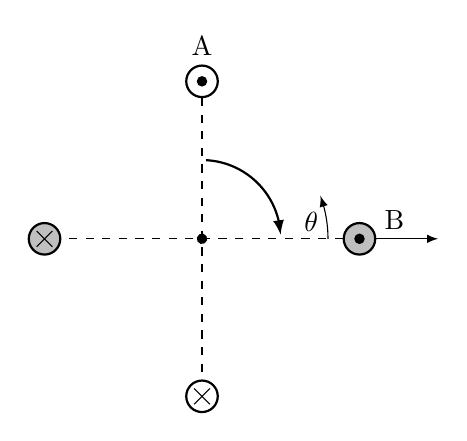
\begin{tikzpicture}[>=latex]
    % flux axis
    \draw[-,dashed] (0,2.2) node[anchor=270]{A};
    \draw[-,dashed] (0:2.2) node[anchor=225]{B};
    \draw[-,dashed] (0,2) -- (0,-2);
    \draw[-,dashed] (0:2.0) -- (180:2.0);
   	\draw[->] (2,0) -- (3,0);
	% out winding
    \filldraw[fill=white,thick] (0,2) circle (0.2);
    \fill (0,2) circle (0.0667);
    \filldraw[fill=lightgray,thick] (0:2.0) circle (0.2);
    \fill (0:2.0) circle (0.0667);
    % in winding
    \filldraw[fill=white,thick] (0,-2) circle (0.2);
    \draw (0.1,-2.1) -- ++(-0.2, 0.2);
    \draw (-0.1,-2.1) -- ++(0.2, 0.2);
    \filldraw[fill=lightgray,thick] (180:2.0) circle (0.2);
    \draw ($(180:2.0) + (0.1,-0.1)$) -- ++(-0.2, 0.2);
    \draw ($(180:2.0) + (-0.1,-0.1)$) -- ++(0.2, 0.2);
	% magnet
	\begin{scope}[rotate=30]
%  		\fill[fill=white] (-1,-0.5) rectangle ++(2,1);
%  		\fill[fill=gray] (-1,-0.5) rectangle ++(1,1);
%  		\draw[-,thick] (-1,-0.5) rectangle ++(2,1);
%   		\draw[] (-0.5,0) node[rotate=30,text=white]{S};
%   		\draw[] (0.5,0) node[rotate=30]{N};
%    	\draw[-,dashdotted] (-3,0) -- (0,0);
%   		\draw[->, very thick] (0,0) -- (2.5,0) node[anchor=210]{d};
%   		\draw[->, very thick] (0,0) -- (0,2.5) node[anchor=300]{q};
%   		\draw[-] (0,0.2) -- (0.2,0.2) -- (0.2,0);
   		\fill (0,0) circle (0.0667);
	\end{scope}
	% rotation
    \draw[->]  (0:1.6)  node[anchor=315]{$\theta$} arc (0:20:1.6);
    % phase to phase arrows
    \draw[->,thick]  (87:1.0)  arc (87:3:1.0);

\end{tikzpicture}
\caption{Phases}
\end{subfigure}
\hspace*{\fill}
\begin{subfigure}[t]{0.45\textwidth}
\begin{circuitikz}[R/.style={european resistor}]
\draw (-3,0) node[anchor=270]{U}
  to[R,l=$A$,f=$i_A$,o-] ++(2,0)
  to[short] ++(1,0) node[anchor=270]{V}
;
\draw (3,0) node[anchor=270]{W}
  to[R,l=$B$,f=$i_B$,o-] ++(-2,0)
  to[short,-o] ++(-1,0)
;

\end{circuitikz}
\caption{2/3 Connection}
\end{subfigure}

\caption[2-Phase w/ 3 Terminals]{2 Phases connected to 3 terminals. Phases are arranged clockwise (physically \unit{-90}{\degree}) with a resultant $\phi = \unit{90}{\degree}$ electrical offset. Unlike a 3-phase system, it is not rotationally symmetrical.}
\label{fig:2ph3ph}
\end{center}
\end{figure}

\begin{figure}[htbp]
\begin{center}
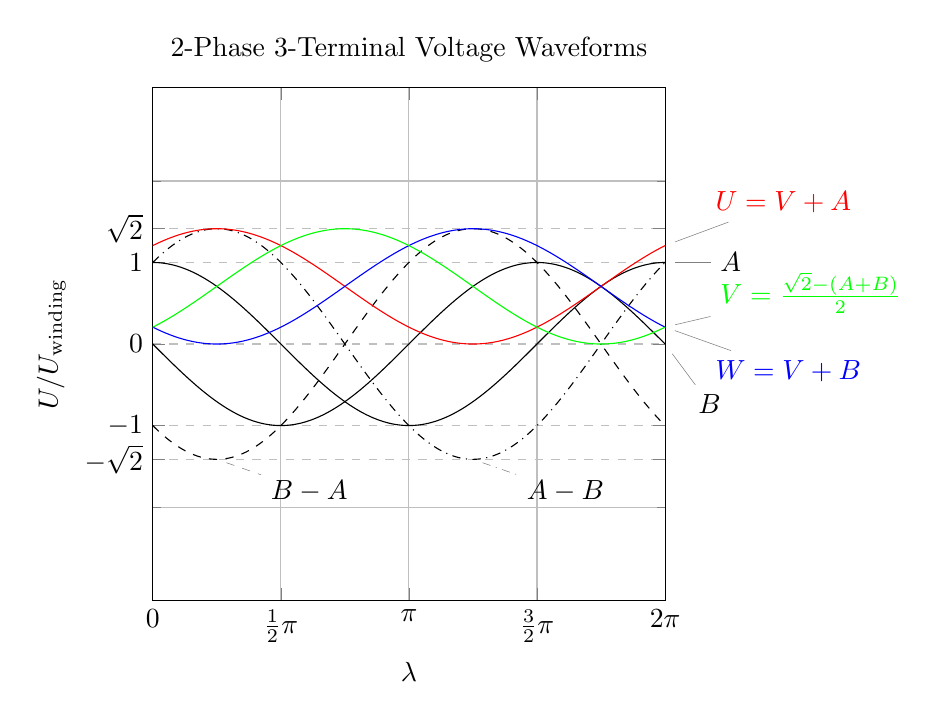
\begin{tikzpicture}[>=latex]
\begin{axis}[
	width=0.667\textwidth,
	height=0.667\textwidth,
	title=2-Phase 3-Terminal Voltage Waveforms, xlabel={$\lambda$}, ylabel={$U / U_{\mathrm{winding}}$}, xmin=0, xmax=2*pi, clip=false,
	axis equal=true,
	enlarge x limits=false,
	xmajorgrids,
	ymajorgrids,
	yminorgrids,
	xtick={0,pi/2, pi, 3/2*pi, 2*pi},
	xticklabels={{$0$}, {$\frac{1}{2}\pi$}, {$\pi$}, {$\frac{3}{2}\pi$}, {$2\pi$}},
	ytick={-sqrt(2), -1, 0, 1, sqrt(2)},
	yticklabels={{$-\sqrt{2}$}, {$-1$}, {$0$}, {$1$}, {$\sqrt{2}$}},
	minor ytick={-2,2},
	major y grid style={dashed},
	]
	\addplot[domain=0:2*pi,samples=361] {cos(deg(x))} node [pos=1,pin=0:{$A$}] {};
	\addplot[domain=0:2*pi,samples=361] {cos(deg(x)+90)} node [pos=1,pin=-60:{$B$}] {};
%	\addplot[domain=0:2*pi,samples=361,dashed] {sqrt(2)*cos(deg(x)+135)} node [pos=1.25/12,pin=-90:{$U_B - U_A$}] {};
	\addplot[domain=0:2*pi,samples=361,dashed] {cos(deg(x)+90) - cos(deg(x)+0)} node [pos=1.25/12,pin=-15:{$B - A$}] {};
	\addplot[domain=0:2*pi,samples=361,dashdotted] {cos(deg(x)+0) - cos(deg(x)+90)} node [pos=7.25/12,pin=-15:{$A - B$}] {};
	% terminal voltage for U
	\addplot[domain=0:2*pi,samples=361,red] {sqrt(2)/2 + 0.5*(cos(deg(x)+0) - cos(deg(x)+90))} node[pos=1,pin=30:{$U = V + A$}]{};
	\addplot[domain=0:2*pi,samples=361,blue] {sqrt(2)/2 + 0.5*(cos(deg(x)+90) - cos(deg(x)+0))} node[pos=1,pin=-30:{$W = V + B$}]{};
	\addplot[domain=0:2*pi,samples=361,green] {sqrt(2)/2 + sqrt(2)/2*(cos(deg(x)-135))} node[pos=1,pin=5:{$V=\frac{ \sqrt{2} - (A + B)}{2}$}]{};
%	\addplot[domain=0:2*pi,samples=361,cyan,dashed] {0.5 * (sqrt(2) - cos(deg(x)+0) - cos(deg(x)+90))};
%	\addplot[domain=0:2*pi,samples=361,cyan,dashed] {sqrt(2)/2 + sqrt(2)/2*(cos(deg(x)-135)) + cos(deg(x)) }; % U via addition of V+U_A
\end{axis}
\end{tikzpicture}

\caption[2/3 Waveforms]{2-phase 3-terminal connection winding and terminal voltage waveforms, showing how terminal voltages are derived from the individual winding and inter-phase voltages.}
\label{fig:waveform23}
\end{center}
\end{figure}


In theory, all motor parameters can be estimated by sequentially turning one half bridge low, while the others are switched high, allowing current to simultaneously flow in at two places, but only out at one. However, the parameter estimation is difficult with noisy values.

\subsection{Full Dynamic Circuit}

\begin{figure}[htbp]
\begin{center}
\begin{circuitikz} 
\draw (0,8) 
  to[R,] ++(0,-2)
  to[normal open switch,] ++(0,-1)
  to[R,] ++(0,-2)
  to[R,] ++(0,-2)
  to[normal open switch,l=$A$] ++(0,-1)
;
\draw (4,8) node[vcc]{U}
  to[R,] ++(0,-2)
  to[normal open switch,] ++(0,-1)
  to[R,] ++(0,-2)
  to[R,] ++(0,-2)
  to[normal open switch,l=$B$] ++(0,-1)
  node[rground]{}
;
\draw (8,8) 
  to[R,l=$R_T$] ++(0,-2)
  to[normal open switch,] ++(0,-1)
  to[R,l=$R_T$] ++(0,-2)
  to[R,l=$R_S$] ++(0,-2)
  to[normal open switch,l=$C$] ++(0,-1)
;
\draw (0,0)
  to[short,-*] ++(4,0)
  to[short] ++(4,0)
;
\draw (0,5)
  to[R,l=$R_P$,*-] ++(2,0)
  to[L,l=$L_P$,] ++(2,0)
  to[R,*-] ++(2,0)
  to[L,-*] ++(2,0)
;
\draw (0,8)
  to[short,-*] ++(4,0)
  to[short] ++(4,0)
;

\end{circuitikz}
\caption[ABBC Driver]{3-Phase Driver with 2-Phase Motor with phase resistance $R_P$ and switching resistance $R_T$ and shunt resistance $R_S$.}
\label{fig:ABBC}
\end{center}
\end{figure}




\begin{figure}[htbp]
\begin{center}
\begin{circuitikz} 
\draw (0,8) 
  to[R,] ++(0,-2)
  to[normal open switch,] ++(0,-1)
  to[R] ++(0,-2)
  to[R,f=$i_A$] ++(0,-2)
  to[short,l=$A$] ++(0,-1)
;
\draw (4,8) node[vcc]{U}
  to[R,f=$i_b$] ++(0,-2)
  to[short,] ++(0,-1)
  to[R,] ++(0,-2)
  to[R,] ++(0,-2)
  to[normal open switch,l=$B$] ++(0,-1)
  node[rground]{}
;
\draw (8,8) 
  to[R,l=$R_T$,f=$i_c$] ++(0,-2)
  to[short,] ++(0,-1)
  to[R,l=$R_T$,] ++(0,-2)
  to[R,l=$R_S$,] ++(0,-2)
  to[normal open switch,l=$C$] ++(0,-1)
;
\draw (0,0)
  to[short,-*] ++(4,0)
  to[short] ++(4,0)
;
\draw (0,5) node[circ,label={[shift={(-0.4,0.0)}]:{$U_a$}}]{}
  to[R,l_=$R_P$,*-] ++(2,0)
  to[L,l_=$L_P$,] ++(2,0) node[circ,label={[shift={(-0.3,0.0)}]:{$U_b$}}]{}
  to[R,-] ++(2,0)
  to[L,-*] ++(2,0) node[circ,label={[shift={(-0.3,0.0)}]:{$U_c$}}]{}
;
\draw (0,8)
  to[short,-*] ++(4,0)
  to[short] ++(4,0)
;

\end{circuitikz}
\caption[ABBC Driver]{Half-Bridge $A$ switched on low, with $B,C$ switched on high creating asymmetric currents across both phases.
}
\label{fig:ABBC-A}
\end{center}
\end{figure}

For the 2-Phase circuit switched as in \cref{fig:ABBC-A} the governing equations with unknowns $i_b,i_c,U_b$ are
\begin{align}
U_b &= L_P \udt i_A + i_A (R_T + R_S + R_P) \\
U-U_b &= i_b R_T \\
U-U_b &= L_P \udt i_c + i_c (R_T + R_P) \\
i_A &= i_b + i_c
\end{align}
and rearranging 
\begin{align}
\udt i_A  &= \frac{U - i_b R_T - i_A (R_T + R_S + R_P)}{L_P} \\
\udt (i_A - i_b)  &= \frac{i_b R_T - (i_A - i_b) (R_T + R_P)}{L_P}
\end{align}
and Laplace transforming
\begin{align}
s I_A(s)  &= \frac{U - I_b(s) R_T - I_A(s) (R_T + R_S + R_P)}{L_P} \\
s \left( I_A(s) - I_b(s) \right) &= \frac{I_b(s) R_T - \left(I_A(s) - I_b(s)\right) (R_T + R_P)}{L_P}
\end{align}
and rearranging
\begin{align}
L_P s I_A(s)  &= U - I_b(s) R_T - I_A(s) (R_T + R_S + R_P) \\
L_P s \left( I_A(s) - I_b(s) \right) &= 2 I_b(s) R_T + I_b(s) R_p - I_A(s) (R_T + R_P)
\end{align}
and again
\begin{align}
R_T I_b(s) &= U - (L_P s + R_T + R_S + R_P) I_A(s)  \\
\left(L_P s + 2 R_T + R_P\right) I_b(s) &= (L_P s + R_T + R_P) I_A(s) 
\end{align}
and combining
\begin{align}
\frac{(L_P s + R_T + R_P)}{L_P s + 2 R_T + R_P} I_A(s)&= \frac{U - (L_P s + R_T + R_S + R_P) I_A(s)}{R_T}
\end{align}
and rearranging
\begin{align}
\left( \frac{(L_P s + R_T + R_P)}{L_P s + 2 R_T + R_P} + \frac{L_P s + R_T + R_S + R_P}{R_T} \right) I_A(s) &= \frac{U}{R_T}
\end{align}
and rearranging
\begin{align}
\left( R_T (L_P s + R_T + R_P) \right. \\
+ &\left (L_P s + R_T + R_S + R_P) (L_P s + 2 R_T + R_P) \right) I_A(s) \\
 = &(L_P s + 2 R_T + R_P) U
\end{align}
expanding
\begin{gather}
\begin{aligned}
\left( R_T L_P s + R_T^2 + R_P R_T \right. \\
+ & L_P^2 s^2 + R_T L_P s + R_S L_P s + R_P L_P s \\
+ & R_T L_P s + 2R_T^2 + R_P R_T \\
+ & R_S L_P s + 2 R_S R_T + R_P R_S\\
+ &\left. R_P L_P s + 2 R_P R_T + R_P^2 \right) I_A(s) \\
 = (L_P s + 2 R_T + R_P) U
\end{aligned}
\end{gather}
simplifying
\begin{gather}
\begin{aligned}
\left( L_P^2 s^2 + 2 R_S L_P s + 2 R_P L_P s + 3 R_T L_P s \right. \\
+ \left. 2 R_S R_T + R_P R_S + R_P^2 + 3 R_T^2 + 4 R_P R_T\right) I_A(s) \\
 = & (L_P s + 2 R_T + R_P) U
\end{aligned}
\end{gather}

\subsection{Resistive Static Circuit}

\begin{figure}[htbp]
\begin{center}
\begin{circuitikz} 
\draw (0,8) 
  to[R,] ++(0,-2)
  to[normal open switch,] ++(0,-1)
  to[R,] ++(0,-2)
  to[R,] ++(0,-2)
  to[normal open switch,l=$A$] ++(0,-1)
;
\draw (4,8) node[vcc]{U}
  to[R,] ++(0,-2)
  to[normal open switch,] ++(0,-1)
  to[R,] ++(0,-2)
  to[R,] ++(0,-2)
  to[normal open switch,l=$B$] ++(0,-1)
  node[rground]{}
;
\draw (8,8) 
  to[R,l=$R_T$] ++(0,-2)
  to[normal open switch,] ++(0,-1)
  to[R,l=$R_T$] ++(0,-2)
  to[R,l=$R_S$] ++(0,-2)
  to[normal open switch,l=$C$] ++(0,-1)
;
\draw (0,0)
  to[short,-*] ++(4,0)
  to[short] ++(4,0)
;
\draw (0,5)
  to[R,l=$R_P$,*-] ++(4,0)
  to[R,*-*] ++(4,0)
;
\draw (0,8)
  to[short,-*] ++(4,0)
  to[short] ++(4,0)
;

\end{circuitikz}
\caption[ABBC Driver Static]{3-Phase Driver with 2-Phase Motor static resistive circuit.}
\label{fig:ABBC-R}
\end{center}
\end{figure}

\begin{figure}[htbp]
\begin{center}
\subfloat[A switched low.]{
\begin{circuitikz} 
\draw (0,8) 
  to[R,] ++(0,-2)
  to[normal open switch,] ++(0,-1)
  to[R] ++(0,-2)
  to[R,f=$i_A$] ++(0,-2)
  to[short,l=$A$] ++(0,-1)
;
\draw (2,8) node[vcc]{U}
  to[R,f=$i_b$] ++(0,-2)
  to[short,] ++(0,-1)
  to[R,] ++(0,-2)
  to[R,] ++(0,-2)
  to[normal open switch,l=$B$] ++(0,-1)
  node[rground]{}
;
\draw (4,8) 
  to[R,l=$R_T$,f=$i_c$] ++(0,-2)
  to[short,] ++(0,-1)
  to[R,l=$R_T$,] ++(0,-2)
  to[R,l=$R_S$,] ++(0,-2)
  to[normal open switch,l=$C$] ++(0,-1)
;
\draw (0,0)
  to[short,-*] ++(2,0)
  to[short] ++(2,0)
;
\draw (0,5)
  to[R,l_=$R_P$,*-*] ++(2,0)
  to[R,-] ++(2,0) 
;
\draw (0,8)
  to[short,-*] ++(2,0)
  to[short] ++(2,0)
;

\end{circuitikz}
}%
~
\subfloat[B switched low.]{
\begin{circuitikz} 
\draw (0,8) 
  to[R,f=$i_a$] ++(0,-2)
  to[short,] ++(0,-1)
  to[R] ++(0,-2)
  to[R,] ++(0,-2)
  to[normal open switch,l=$A$] ++(0,-1)
;
\draw (2,8) node[vcc]{U}
  to[R,] ++(0,-2)
  to[normal open switch,] ++(0,-1)
  to[R,] ++(0,-2)
  to[R,f=$i_B$] ++(0,-2)
  to[short,l=$B$] ++(0,-1)
  node[rground]{}
;
\draw (4,8) 
  to[R,l=$R_T$,f=$i_c$] ++(0,-2)
  to[short,] ++(0,-1)
  to[R,l=$R_T$,] ++(0,-2)
  to[R,l=$R_S$,] ++(0,-2)
  to[normal open switch,l=$C$] ++(0,-1)
;
\draw (0,0)
  to[short,-*] ++(2,0)
  to[short] ++(2,0)
;
\draw (0,5)
  to[R,l_=$R_P$,*-*] ++(2,0)
  to[R,-] ++(2,0) 
;
\draw (0,8)
  to[short,-*] ++(2,0)
  to[short] ++(2,0)
;

\end{circuitikz}
}
\caption[ABBC-RAB]{Resistive Half-Bridge switched low on $A,B$ phases, respectively.
}
\label{fig:ABBC-RAB}
\end{center}
\end{figure}

For the 2-Phase circuit switched as in \cref{fig:ABBC-RAB} the measureable resistances are
\begin{gather}
\begin{aligned}
R_A &= R_S + R_T + R_P + \frac{R_T (R_T + R_P)}{2 R_T + R_P} \\
R_B &= R_S + R_T + \frac{R_T + R_P}{2}
\end{aligned}
\end{gather}
which allows us to solve for $R_T, R_P$ with $R_S$ being known:
\begin{gather}
\begin{aligned}
(2 R_T + R_P) (R_A - R_S - R_T - R_P) &= R_T (R_T + R_P) \\
R_P &= 2 R_B - 2 R_S - 3 R_T
\end{aligned}
\end{gather}
and combining the two equations to solve for $R_T$
\begin{gather}
\begin{aligned}
(2 R_B - 2 R_S - R_T) (R_A + R_S + 2 R_T - 2 R_B) &= R_T (2 R_B - 2 R_S - 2 R_T) \\
2 R_A R_B + 2 R_B R_S + 4 R_B R_T - 4 R_B^2 \\
 - 2 R_A R_S - 2 R_S^2 - 4 R_S R_T + 4 R_B R_S\\
 - R_A R_T - R_S R_T - 2 R_T^2 + 2R_B R_T &= 2 R_B R_T - 2 R_S R_T - 2 R_T^2 \\
2 R_A R_B - 4 R_B^2 - 2 R_A R_S - 2 R_S^2 + 6 R_B R_S &= R_A R_T + 3 R_S R_T - 4 R_B R_T\\
2 \frac{ R_A R_B - 2 R_B^2 - R_A R_S - R_S^2 + 3 R_B R_S}{R_A + 3 R_S- 4 R_B} &= R_T\\
2 \frac{ 2 R_B^2 - R_A R_B  + R_A R_S - 3 R_B R_S + R_S^2}{4 R_B - R_A - 3 R_S} &= R_T\\
\end{aligned}
\end{gather}
and for $R_P$
\begin{gather}
\begin{aligned}
2 \frac{ 2 R_B^2 - R_A R_B  + R_A R_S - 3 R_B R_S + R_S^2}{4 R_B - R_A - 3 R_S} &= \frac{R_P - 2 R_B + 2 R_S}{3} \\
\frac{ 12 R_B^2 - 6 R_A R_B  + 6 R_A R_S - 18 R_B R_S + 6 R_S^2}{4 R_B - R_A - 3 R_S} + 2 R_B - 2 R_S &= R_P \\
\frac{ 20 R_B^2 - 8 R_A R_B  + 8 R_A R_S - 32 R_B R_S + 12 R_S^2}{4 R_B - R_A - 3 R_S} &= R_P \\
4 \frac{ 5 R_B^2 - 2 R_A R_B  + 2 R_A R_S - 8 R_B R_S + 3 R_S^2}{4 R_B - R_A - 3 R_S} &= R_P
\end{aligned}
\end{gather}

\subsection{Single Current Path}

System identification  with only one active high and low switch at a time, and the third half-bridge being disabled, results in simpler equations than having two active high switches:
\begin{gather}
\begin{aligned}
R_{AB} = R_{BC} &= R_P + 2 R_T + R_S \\
R_{AC} &= 2 R_P + 2 R_T + R_S \\
\end{aligned}
\end{gather}

\subsection{2-Phase Driving}

Because the 2 phases share a common point, the maximum available voltage is limited to less than the line voltage. It is assumed that the phases are driven sinusoidally with a $\frac{\pi}{2}$ phase shift.

With a naive approach of keeping the center point at half the nominal voltage, only half the nominal voltage is available for each phase. Moving the midpoint, too, allows us to increase phase voltage to $U_P = \sqrt{2} U$, with the following waveforms:
\begin{gather}
\begin{aligned}
U_{A} &= \frac{\cos x}{\sqrt{2}} \\
U_{C} &= \frac{\sin x}{\sqrt{2}} \\
U_{B} &= \frac{\cos x + \sin x}{4} = \frac{\cos \left(x - \frac{\pi}{4}\right)}{2 \sqrt{2}}
\end{aligned}
\end{gather}
and PWM
\begin{gather}
\begin{aligned}
D_{A} &= U_{B} + U_{A} \\
D_{B} &= U_{B} \\
D_{C} &= U_{B} + U_{C}
\end{aligned}
\end{gather}

The physical limiting condition to observe is that 
\begin{gather}
\begin{aligned}
\forall \left( U_{A}+U_{B} \right) &\leq U_P
\end{aligned}
\end{gather}

\section{Motor Model}

\subsection{DC Motor State Equation}

The electrical and mechanical DC motor model with the parameters of  electrical motor constant $k_e$, rotor inertia $J$, dynamic friction $k_d$, and disturbance torque $\Gamma_d$:

\begin{gather}
\begin{aligned}
L\frac{\ud }{\ud t} \imath&= U - R \imath - k_e \omega \\
J \frac{\ud }{\ud t} \omega &= k_e \imath - k_d \omega - \Gamma_d \\
\frac{\ud}{\ud t} x &= \omega
\end{aligned}
\end{gather}

\subsection{2-Phase Stepper Motor Model}

The stepper motor model is similar to DC motor model, but takes into account the currents flowing in each phase. The number of steps per revolution is
\begin{gather}
\begin{aligned}
S &= 2 \cdot m \cdot n
\end{aligned}
\end{gather}
where $n$ is the number of pole-pairs and $m$ is the number of phases. For a typical \unit{1.8}{\degree} per step for $S=200$ and $m=2$, it follows that there are $n=50$ pole-pairs.

Assuming a sinusoidal magnetic characteristic the torque contribution from each phase is
\begin{gather}
\begin{aligned}
\tau_j &= k_m \sin \left( n \theta_m + \phi_{0j}\right) \cdot \imath_j
\end{aligned}
\end{gather}
where $\theta_m$ is the mechanical angle of the rotor and $\phi_{0j}$ is the phase offset. The model is very similar to the DC motor\footnote{we use a 2-phase PM motor model} except that the torque is the sum of the phase torques
\begin{gather}
\begin{aligned}
J \frac{\partial }{\partial t} \omega &= \sum_j\tau_j - k_d \omega_m - \Gamma_d \\
\sum_j \tau_j &= k_m I \sin \phi_m
\end{aligned}
\end{gather}
The current is a function of the applied voltage and motor back-EMF\footnote{The electrical equations are valid for any number of phases}
\begin{gather}
\begin{aligned}
\label{eq:motphase} U_j &= E_j + R \imath_j + L \frac{\partial \imath_j}{\partial t} \\
E_j &= k_e \omega_m \cos \left( n \theta_m + \phi_{0j} \right) = k_e \omega_m \cos \left( \theta_{ej} + \phi_m \right)
\end{aligned}
\end{gather}
Further ignoring the winding offsets, all phases behave the same. The only unknowns in \cref{eq:motphase} after electrical parameter identification of $R,L$ are $k_e$, and $\phi_m$, as $U$, $\imath$, and $\omega_m$ are directly observed.

It is noteworthy that $E$ is phase-shifted by $\phi_m$, but it's magnitude is independent of it, thus the RMS value $E_{\mathrm{RMS}}$ of $E$ is independent of $\phi_m$ being
\begin{gather}
\begin{aligned}
E_{\mathrm{RMS}} &= \frac{1}{\sqrt{2}} k_e \omega_m
\end{aligned}
\end{gather}

For a constant $\omega$, we can look at the phase relationships
\begin{gather}
\begin{aligned}
\mathbf{E} &= \mathbf{U} - \mathbf{Z} \mathbf{\imath} \\
k_e \omega_m \cos \left( \theta_{e} + \phi_m \right) &= U \cos(\theta_{e} + \phi_e) - R I \cos(\theta_e) - LI \sin(\theta_e) \\
k_e \omega_m e^{j \phi_m}  &= U e^{j \phi_e} - R I - LI e^{j \pi/2}
\end{aligned}
\end{gather}

%Thus
%\begin{gather}
%\begin{aligned}
%U_j &= k_m \cos \left( n \theta_m + \phi_{0j} \right) \omega_m + R I \cos \left( \theta_e + \phi_{0j} \right) - L I \sin \left( \theta_e + \phi_{0j} \right) \\
%\phi_Z &= \arctan\left(\frac{L}{R}\right) \\
%\phi_m &= n\theta_m - \theta_e \\
%U_j &= k_m \omega_m\cos \left( n \theta_m + \phi_{0j} \right) + Z I \cos \left( n\theta_m + \phi_{0j} + \phi_Z - \phi_m \right) \\
%\tan \varphi &= \frac{ZI\sin(\phi_Z-\phi_m)}{k_m \omega_m + ZI\cos(\phi_Z-\phi_m)} \\
%U_j &= \sqrt{ k_m^2\omega_m^2 + Z^2I^2  + 2 k_m \omega_m Z I \cos \left(\phi_m - \phi_Z \right)} \cos \left( n \theta_m + \phi_{0j} + \varphi \right)
%\end{aligned}
%\end{gather}

\subsubsection{Parameter Estimation}

\begin{table}[htbp]
\caption{Motor parameter estimation steps.}
\begin{center}
\begin{tabular}{llp{0.5\textwidth}} \toprule
 \multicolumn{2}{l}{Parameter} & Estimation Condition \\
\midrule
$R$ & winding resistance & static current\\
$L$ & winding inductance & dynamic current\\
$k_e$ & el.\ motor constant & constant speed\\
$k_d$ & dynamic friction & variable speed\\
$k_s$ & static friction & ???\\
? & encoder offset & variable position\\
$t_?$ & encoder delay & ???\\
$\phi_m$ & load angle & constant speed \\
\bottomrule
\end{tabular}
\end{center}
\label{tab:paramest}
\end{table}%


$R,L$ can be determined by mechanically static (no significant rotation) tests, as they are purely a function of the electrical circuit. 

The back-EMF can be determined through change of $i_{\textrm{RMS}}$ when applying a constant-voltage with different speeds. Though $U, \imath, E$ are all synchronous, they will not be in the same phase.
\begin{gather}
\begin{aligned}
U_j &= \sqrt{ k_m^2\omega_m^2 + Z^2I^2  + 2 k_m \omega_m Z I \cos \left(\phi_m - \phi_Z \right)} \cos \left( n \theta_m + \phi_{0j} + \varphi \right) \\
U_{\textrm{RMS}} &= \frac{1}{\sqrt{2}} \sqrt{ k_m^2\omega_m^2 + Z^2I^2  + 2 k_m \omega_m Z I \cos \left( \phi_m - \phi_Z \right)}
\end{aligned}
\end{gather}
$k_m$ and $\phi_m$ are unknowns. $\phi_m$ depends on the motor's load condition, but can be eliminated in approximations. For $\omega = 0$, this is just the familiar
\begin{gather}
\begin{aligned}
U_{\textrm{RMS}} &= \frac{1}{\sqrt{2}} ZI
\end{aligned}
\end{gather}
and for $\omega \gg 0$, as $\phi_m$ approaches \unit{90}{\degree}
\begin{gather}
\begin{aligned}
U_{\textrm{RMS}} &\approx \frac{1}{\sqrt{2}} k_m \omega_m
\end{aligned}
\end{gather}

Assuming viscous friction only, is there a speed with a minimum current for constant voltage pwm before stall due to the interaction of EMF and phase lag?
\begin{gather}
\begin{aligned}
k_m I \sin \phi_m &= k_d \omega_m \\
\sin \phi_m &= \frac{k_d \omega_m}{k_m I} \\
2 U^2_{\textrm{RMS}} &= k_m^2\omega_m^2 + Z^2I^2  + 2 k_m \omega_m Z I \cos \left( \phi_m - \phi_Z \right)\\
0 & = Z^2I^2  + 2 k_m \omega_m Z I \cos \left( \phi_m - \phi_Z \right) + k_m^2\omega_m^2 - 2 U^2_{\textrm{RMS}} \\
I &= \frac{-2 k_m \omega_m Z \cos \left( \phi_m - \phi_Z \right) \pm \sqrt{4 k^2_m \omega^2_m Z^2 \cos^2 \left( \phi_m - \phi_Z \right) - 4 Z^2 \left( k_m^2\omega_m^2 - 2 U^2_{\textrm{RMS}} \right)}}{2 Z^2} \\
I &= \frac{-k_m \omega_m \cos \left( \phi_m - \phi_Z \right) \pm \sqrt{k^2_m \omega^2_m \left(\cos^2 \left( \phi_m - \phi_Z \right) - 1\right) + 2 U^2_{\textrm{RMS}} }}{Z} \\
I &= \frac{-k_m \omega_m \cos \left( \phi_m - \phi_Z \right) \pm \sqrt{k^2_m \omega^2_m \sin^2 \left( \phi_m - \phi_Z \right) + 2 U^2_{\textrm{RMS}} }}{Z}
\end{aligned}
\end{gather}
splitting $\cos \left( \phi_m - \phi_Z \right)$ via harmonic addition
\begin{gather}
\begin{aligned}
\cos \left( \phi_m - \phi_Z \right)&= \frac{1}{Z} \left( R\cos \phi_m + L \sin \phi_m \right) \\
%- \phi_Z &= \arctan \left( - \frac{L}{R} \right) \\
\rho &= \frac{k_d \omega_m}{k_m I} \\
\cos \left( \phi_m - \phi_Z \right)&= \frac{1}{Z} \left( R \sqrt{1-\rho^2} + L \rho \right) \\
2 k_m \omega_m I \left( R \sqrt{1-\rho^2} + L \rho \right) &= 2 k_d \omega_m^2 L + 2 k_m \omega_m I R \sqrt{1-\rho^2}\\
&= 2 k_d \omega_m^2 L + 2 k_m \omega_m R \sqrt{I^2-I\frac{k_d^2 \omega_m^2}{k_m^2}} \\
2 k_m \omega_m R \sqrt{I^2-I\frac{k_d^2 \omega_m^2}{k_m^2}}& = 2 U^2_{\textrm{RMS}} -k_m^2\omega_m^2 - Z^2I^2  - 2 k_d \omega_m^2 L \\
\end{aligned}
\end{gather}
differentiating wrt $\omega$ to find minima/maxima
\begin{gather}
\begin{aligned}
\frac{\partial}{\partial \omega_m} 2 k_m \omega_m R \sqrt{I^2-I\frac{k_d^2 \omega_m^2}{k_m^2}}& = \frac{\partial}{\partial \omega_m} \left( -k_m^2\omega_m^2 - 2 k_d \omega_m^2 L \right)\\
2 k_m R \sqrt{I^2-I\frac{k_d^2 \omega_m^2}{k_m^2}} +  2 R  \left(I^2-I\frac{k_d^2 \omega_m^2}{k_m^2}\right)^{-\frac{1}{2}} I\frac{k_d^2 \omega_m^2}{k_m} & =   - 2k_m^2\omega_m - 4 k_d \omega_m L \\
R \sqrt{k_m^2 I^2-I k_d^2 \omega_m^2} +  R  \left(k_m^2 I^2 - I k_d^2 \omega_m^2\right)^{-\frac{1}{2}} I k_d^2 \omega_m^2  & = - k_m^2\omega_m - 2 k_d \omega_m L \\
\end{aligned}
\end{gather}
\begin{gather}
\begin{aligned}
R \left(k_m^2 I^2 - I k_d^2 \omega_m^2 \right) +  R I k_d^2 \omega_m^2  & = - R \sqrt{k_m^2 I^2-I k_d^2 \omega_m^2} \left(k_m^2\omega_m - 2 k_d \omega_m L \right) \\
R k_m^2 I^2  & = - R \sqrt{k_m^2 I^2-I k_d^2 \omega_m^2} \left(k_m^2\omega_m - 2 k_d \omega_m L \right) \\
R^2 k_m^4 I^4  & = R^2 \left( k_m^2 I^2-I k_d^2 \omega_m^2 \right) \left(k_m^2\omega_m - 2 k_d \omega_m L \right)^2 \\
k_m^4 I^3  & = \omega_m^2 \left( k_m^2 I - k_d^2 \omega_m^2 \right) \left(k_m^2 - 2 k_d \right)^2 \\
k_m^4 I^3   - \omega_m^2 k_m^2 \left(k_m^2 - 2 k_d \right)^2 I & = - k_d^2 \omega_m^4  \left(k_m^2 - 2 k_d \right)^2 \\
\end{aligned}
\end{gather}
is a depressed cubic that can be solved with Cardano's formula
\begin{gather}
\begin{aligned}
k_m^4 I^3 - \omega_m^2 k_m^2 \left(k_m^2 - 2 k_d \right)^2 I & = - k_d^2 \omega_m^4  \left(k_m^2 - 2 k_d \right)^2 \\
p &= - \omega_m^2 k_m^2 \left(k_m^2 - 2 k_d \right)^2 \\
q &= \omega_m^4  \left(k_m^2 - 2 k_d \right)^2 \\
q^2/4 + p^3/27 &= \frac{1}{4} k_d^4 \omega_m^8  \left(k_m^2 - 2 k_d \right)^4 - \frac{1}{3^3} \omega_m^6 k_m^6 \left(k_m^2 - 2 k_d \right)^6 \\
q^2/4 + p^3/27 &= \omega_m^6 \left(k_m^2 - 2 k_d \right)^4 \left(\frac{1}{4}k_d^4 \omega_m^2   - \frac{1}{3^3} k_m^6 \left(k_m^2 - 2 k_d \right)^2 \right) \\
\sqrt{q^2/4 + p^3/27} &= \omega_m^3 \left(k_m^2 - 2 k_d \right)^2 \sqrt{\frac{1}{4}k_d^4 \omega_m^2- \frac{1}{3^3} k_m^6 \left(k_m^2 - 2 k_d \right)^2 } \\
\end{aligned}
\end{gather}

solving for $\omega$
\begin{gather}
\begin{aligned}
0 &= k_d^2 \omega_m^4  \left(k_m^2 - 2 k_d \right)^2   - \omega_m^2 k_m^2 \left(k_m^2 - 2 k_d \right)^2 I + k_m^4 I^3 \\
\end{aligned}
\end{gather}



\begin{gather}
\begin{aligned}
\sin \left( \phi_m - \phi_Z \right)&= \sin \phi_m \cos \phi_Z - \cos \phi_m \sin \phi_Z \\
\sin^2 \left( \phi_m - \phi_Z \right)&= \sin^2 \phi_m \cos^2 \phi_Z + \cos^2 \phi_m \sin^2 \phi_Z - 2 \sin \phi_m \cos \phi_Z \cos \phi_m \sin \phi_Z\\
\rho &= \frac{k_d \omega_m}{k_m I} \\
\sin^2 \left( \phi_m - \phi_Z \right)&= \rho^2 \cos^2 \phi_Z + \left( 1-\rho^2 \right) \sin^2 \phi_Z - 2 \rho \cos \phi_Z \sqrt{1-\rho^2} \sin \phi_Z
\end{aligned}
\end{gather}
aproximating $\phi_Z \approx 0$
\begin{gather}
\begin{aligned}
\sin^2 \left( \phi_m - \phi_Z \right)&= \rho^2 \\
%\sin^2 \left( \phi_m - \phi_Z \right)&= \sin^2 \phi_m \cos^2 \phi_Z + \left(1 - \sin^2 \phi_m \right) \sin^2 \phi_Z - 2 \sin \phi_m \cos \phi_Z \cos \phi_m \sin \phi_Z\\
 I &= \frac{\mp k_m \omega_m \left(1 - \sin^2 \left( \phi_m - \phi_Z \right) \right) \pm \sqrt{k^2_m \omega^2_m \sin^2 \left( \phi_m - \phi_Z \right) + 2 U^2_{\textrm{RMS}} }}{Z} \\
 I &= \frac{\mp k_m \omega_m \left(1 - \rho^2 \right) \pm \sqrt{k^2_m \omega^2_m \rho^2 + 2 U^2_{\textrm{RMS}} }}{Z}
\end{aligned}
\end{gather}

\subsection{Observability}

Ideally, our motor model perfectly captures all relevant properties needed to control torque, velocity, and positioning. However, that will never truly be the case, so we rely on estimating parameters for known relationships, and accounting for unknowns with black-box parameters.

We typically treat a motor model as static, and do not change the "fixed" parameters while we're controlling the motor, and only try to account for some variables like a varying or unknown load.

Apart from the electrical motor itself, a given machine might allow further modeling to increase the model's fidelity, and thus control accuracy and precision. For example, a robot arm's mass, inertia, and the influence of gravity can be modeled in the controller instead of assuming a black-box load.

As we increase the number of parameters, it might not be possible to estimate parameters, even for known configurations, if we don't have the required sensors.

\subsection{Parameter Estimation through a Kalman Filter}

If we model the motor parameters as state variables of a Kalman Filter, the filter's process and measurement covariance matrices $\mQ, \mR$ should include all the information necessary to improve parameter estimates at runtime, as long as we can approximate them well enough.

\section{Motor Discovery Implementation}


The implementation / parameter estimation is implemented as:
\begin{enumerate}
\item For each bridge, do a static test
    \begin{enumerate}
    \item apply large single-phase current to align rotor, wait to settle down mechanically, then zero current
    \item apply full voltage and measure current and measure current ramp to threshold current
    \item apply steady-state low duty cycle PWM and measure current for resistance estimate
    \end{enumerate}
\end{enumerate}


\section{Position Estimation}

\subsection{Discrete Kalman Filter}

\subsubsection{Difference Equation}

Variable names after \cite{kalman-tut} with slight adjustments. The discrete stochastic time-variant system is described by
\begin{gather}
\begin{aligned}
\vx_k &= \mA_{k} \vx_{k-1} +  \mB_{k} \vu_{k-1} + \vw_{k-1} \\
\vz_k &= \mH_k \vx_k + \vv_k
\end{aligned}
\end{gather}
where \vx\ is the state vector, \vu\ is the input vector, \vz\ is the observation vector, and \vw\ and \vv\ are the process and measurement noise vector vectors, respectively, for a given time step $k$.

$\mH$ maps the state to the observable variables, and features prominently in the Kalman Filter equations.

The noise vectors are defined by the corresponding covariance matrices $\mQ_k$ and $\mR_k$. The state covariance matrix is $\mP_k$.

\subsubsection{Canonical Kalman Filter Update}

The first part of the update is prediction
\begin{gather}
\begin{aligned}
\vx^-_k &= \mA \vx^+_{k-1} +  \mB \vu_{k-1} \\
\mP^-_k &= \mA\mP^+_{k-1}\mA^T + \mQ
\end{aligned}
\end{gather}
which results in the \em a-priori \em (as in before measurement) estimates of $\vx^-, \mP^-$. The second part is the correction through measurement
\begin{gather}
\begin{aligned}
\mK &= \mP^-_k\mH^T\left( \mH \mP^-_k \mH^T + \mR \right)^{-1}\\
\vx^+_k &= \vx^-_k + \mK \left(\vz_k - \mH\vx^-_k \right)\\
\end{aligned}
\end{gather}
resulting in the \em Kalman Gain \em $\mK$, and \em a-posteriori \em (post measurement) estimates of the state vector $\vx^+$. In this form, the computation of $\mK$ requires a matrix inversion. If the process and measurement noise covariance matrices are constant, the inversion can be avoided by pre-computing the state covariance matrix $\mP$ with the Ricatti Equation. In our case, however, both $\mQ$ and $\mR$ are time-dependent.

The final step is updating the state covariance $\mP$, which for the optimal Kalman gain is simplified
\begin{gather}
\begin{aligned}
\mP^+_k &= \left( \mI - \mK \mH \right) \mP^-_k
\end{aligned}
\end{gather}
or the more numerically robust \em Joseph form,\em which preserves symmetry even in case of numerical rounding errors:
\begin{gather}
\begin{aligned}
\mP^+_k &= \left( \mI - \mK \mH \right) \mP^-_k \left( \mI - \mK \mH \right)^T + \mK \mR \mK^T
\end{aligned}
\end{gather}


\subsubsection{Sequential Kalman Filter}

The sequential Kalman filter applies measurements one at a time, instead of all at once, resulting in some numerical simplification.

Reformulating the correction step in terms of the measurement prediction covariance $\mS$:
\begin{gather}
\begin{aligned}
\mS &= \mH \mP^-_k \mH^T + \mR \\
\mK &= \mP^-_k\mH^T \mS^{-1}
\end{aligned}
\end{gather}
allows us to see that for each scalar measurement $z_i$, with scalar covariance $r_i$ the measurement prediction covariance also becomes scalar, and thus
\begin{gather}
\begin{aligned}
s_i &= \mH \mP^-_k \mH^T + r_i \\
\mK_i &= \frac{\mP^-_k\mH^T}{s_i}
\end{aligned}
\end{gather}
for each measurement.

\subsubsection{Simplest Approximation Difference Equations}

In the simplest possible form, the motor can be treated as an inertial mass without outside forces, eg.{} it having constant speed.

\begin{gather}
\begin{aligned}
\omega &= \frac{\ud}{\ud t} x
\end{aligned}
\end{gather}

This is a useful approximation if further motor parameters that link the electrical and mechanical models are unknown, but has the big drawback that changes in speed cannot be modeled well. Therefore, this model is only useful to determine motor position and speed from the position encoder during system identification, but not during regular operation.

The mechanical position $x$ of the motor and its speed $\omega$ compromise the state vector. There are no inputs, and the only available measurement is the measured position $x'$:
\begin{gather}
\begin{aligned}
\vx &= \left(
\begin{array}{c}
      x  \\
 \omega \\
%\ddot{x}   
\end{array}
\right) \\
%\vu &= \left(
%\begin{array}{c}
%      \imath
%\end{array}
%\right) \\
\vz &= \left(
\begin{array}{c}
      x'
\end{array}
\right)
\end{aligned}
\end{gather}
The update/correction matrices depend only on the time step size $h$:
\begin{gather}
\begin{aligned}
\mA &= \left(
\begin{array}{cc}
 1 & h \\
 0 & 1 \\
\end{array}
\right) \\
%\mB &= \left(
%\begin{array}{c}
% k_T \frac{h^2}{2} \\
% k_T h   
%\end{array}
%\right) \\
\mH &= \left(
\begin{array}{c c}
 1 & 0
\end{array}
\right).
\end{aligned}
\end{gather}
Without inputs, $\mB\vu = 0$ and can be ignored.

The covariance matrices are the most difficult to determine. We need to take into account the effects of the applied voltage $U$ and/or current $\imath$, and balance the model and measurement covariances to get a stable prediction, but also a fast enough reaction, though such a filter will invariable react more slowly to changes than a more complete model. In addition to $h$, we might also consider the change in input voltage $\frac{\ud}{\ud t} U$ and time since the last observation $\lambda$
\begin{gather}
\begin{aligned}
%\mP &= \left(
%\begin{array}{cc}
% ? & 0 \\
% 0 & ? \\
%\end{array}
%\right) \\
\mQ &= \left(
\begin{array}{cc}
 \left( k_{Q1} h \right)^2 & 0 \\
 0 & \left( k_{Q2} h \right)^2
\end{array}
\right) \\
\mR &= \left(
\begin{array}{c}
 \left( k_{R1} + k_{R2} \lambda + k_{R3} \omega \lambda \right)^2\\
\end{array}
\right)
\end{aligned}
\end{gather}
For $\mR$, we will have a noise figure from the sensor to determine $k_{R1}$. $k_{R2}$ expresses how much we trust the measurement as time goes on without further information, and $k_{R2}$ expresses uncertainty it terms of rotational speed.

If the motor that isn't being driven, what is the expected amount we expect it to move? For a stepper motor, we expect it might clog to the next full step. If it is moving, and we expect it to continue so without further input, it will have moved $\omega \lambda$ plus some unmodeled effect from potential friction. 

The uncertainty in the process might quantified by taking into account potential forces that are not accounted for in the model. Neglecting external forces, we have control over our target speed $\omega$ and the acceleration $\alpha_{\textrm{max}}$.

For a scalar $R$, due to only having a single observed variable, $\mK$ can be calculated straight-forwardly without a matrix inversion.

\begin{table}[htbp]
\caption{Covariance parameters for constant speed motor model.}
\begin{center}
\begin{tabular}{llp{0.5\textwidth}} \toprule
 Parameter & Value & Comment \\
\midrule
$k_{Q1}$ & $0.2\pi$ & \unit{10}{\%} of $\alpha_{\textrm{max}}$ as unmodeled disturbance\\
$k_{Q2}$ & $2\pi$ & larger uncertainty in speed, due it being derived from position\\
$k_{R1}$ & $0.0222$  & ONL $\sigma = \unit{0.068}{\degree}$ + INL $ = \unit{1.2}{\degree}$\\
$k_{R2}$ & $2\pi$ & $\alpha_{\textrm{max}} = \unit{2\pi}{\radian\per\second\squared}$ acc limit \\
$k_{R3}$ & $0$ & assuming measurement is compensated by speed est. \\
\bottomrule
\end{tabular}
\end{center}
\label{tab:cov-params-const-speed}
\end{table}%


\section{Cogging}

PMSM type motors, including BLDCs, exhibit a phenomenon known as cogging: because of the permanent magnets, even when unenergized, the rotor experience a non-constant torque as it rotates, pulling it towards certain positions that maximize magnetic flux between the rotor and the stator.

\subsection{Cogging Model}

\begin{figure}[htbp]
\begin{center}
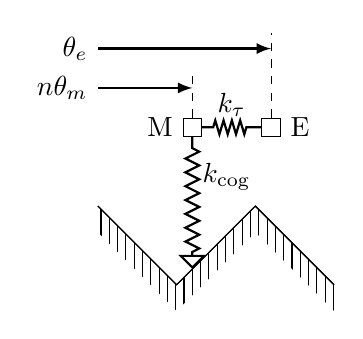
\begin{tikzpicture}[>=latex]
	\tikzstyle{spring}=[thick,decorate,decoration={zigzag,pre length=4,post length=4,segment length=6}]
	\tikzstyle{ground}=[fill,pattern=vertical lines,draw=none,minimum width=0.75cm,minimum height=0.3cm,inner sep=0pt,outer sep=0pt]

	% axis
	\draw[thick,->] (-1,3) node[anchor=east]{$\theta_e$} -- ++( 2.2, 0);
	\draw[thick,->] (-1,2.5) node[anchor=east]{$n\theta_m$} -- ++( 1.2, 0);

	% connecting node
	\node[shape=rectangle,draw,minimum size=0.05cm] (A) at (0.2,2) {};
	\node[shape=rectangle,draw] (B) at (1.2,2) {};
	\draw[dashed] (B.north) -- ( 1.2, 3.2);
	\draw[dashed] (A.north) -- ( 0.2, 2.7);
	\draw (A.west) node[anchor=east] {M};
	\draw (B.east) node[anchor=west] {E};
    % pin
	\draw (-1,1) -- ++( 1, -1) -- ++( 1, 1) -- ++( 1, -1);
    \draw[spring,>=open triangle 90,->,thick,decoration={zigzag,segment length=5}] (A.south) -- (0.2,0.2) node[pos=0.3,right] {$k_{\mathrm{cog}}$};
    % torque
    \draw[spring,-,thick,decoration={zigzag,segment length=3}] (A.east) -- (B.west) node[pos=0.5,above] {$k_{\tau}$};
%   	\draw[->] (-3,0) -- (3,0); % node[anchor=south west] {$\mathbf{\mu}$};
	% notches
	\fill[ground] (-1,1) -- ++( 1, -1) -- ++( 1, 1) -- ++( 1, -1) -- ++( 0.0, -0.333) -- ++( -1, 1) -- ++( -1, -1)  -- ++( -1, 1) -- cycle;
	\draw (-1,1) -- ++( 1, -1) -- ++( 1, 1) -- ++( 1, -1);

\end{tikzpicture}
\caption[Linear Cogging Model]{Linear cogging model similar to a pin-tumbler lock. The pin is connected to (M) with a compression spring, while (M) is connected to (E) with a tension spring. (M) represents the mechanical movement, while (E) represents the magnetic field rotation. $\theta_e - n\theta_m$ is the torque angle, and the higher it is, the more force is applied towards compressing the pin spring, and thus to move (M) towards (E).}
\label{fig:cogmod}
\end{center}
\end{figure}

A linear cogging model as shown in \cref{fig:cogmod} can work as first approximation, and highlights the main problem with cogging compensation: for a rotor position $\theta_m$ close the inflection point between one cog and the next, hysteresis is introduced in the electrical angle $\theta_e$ for the same mechanical position, depending on which direction the transition is approached from.

The good news is that under load, the instability around the inflection is reduced in effect.

The cogging torque must be compensated by either modulating the motor current amplitude and phase. Based on the single phase winding model \cref{eq:singlephase}, the speed of current change
\begin{gather}
\begin{aligned}
\label{eq:didt-winding} 
\frac{\partial \imath}{\partial t} = \frac{U - E - R \imath}{L}
\end{aligned}
\end{gather}
can tell us how fast the system can react for a given operating point. The equation shows that the available voltage $U_d = U - E - R i$ is the only variable parameter that determines ${\partial \imath} / {\partial t}$.

Both phase and amplitude modulation are limited by ${\partial \imath} / {\partial t}$, and in practice it seems like it should make sense to keep the torque angle at a maximum for most effective torque modulation, but cogging introduces non-linear effects. 

\subsubsection{Characterizing Cogging}

Cogging typically pulls a hybrid or permanent magnet motor into the next step position, which would be the same as fully energizing the corresponding motor phase. For a 3-phase configuration from \cref{fig:star}, as shown in the phase diagram \cref{fig:waveform3}, these rest points correspond to $\lambda_k = \frac{1}{3}\pi k$. Moving the current phase away from the rest point by $\Delta \theta_e$, the mechanical phase $\Delta n\theta_m$ will move a reduced amount, due to the cogging torque holding the rotor in place.

\begin{figure}[htbp]
\begin{center}
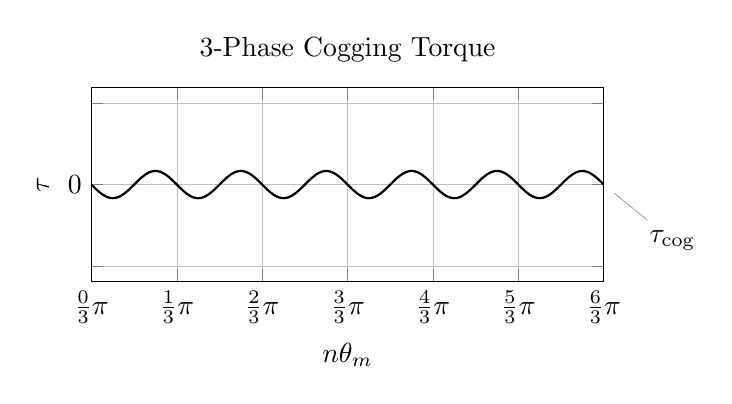
\begin{tikzpicture}[>=latex]
	\begin{axis}[
	width=0.667\textwidth,
	height=0.333\textwidth,
	title=3-Phase Cogging Torque, xlabel={$n\theta_m$}, ylabel={$\tau$}, xmin=0, xmax=2*pi, clip=false,
	axis equal=true,
	enlarge x limits=false,
	xmajorgrids,
	ymajorgrids,
	yminorgrids,
	xtick={0,pi/3, 2*pi/3, pi, 4/3*pi, 5/3*pi, 2*pi},
	xticklabels={{$\frac{0}{3}\pi$}, {$\frac{1}{3}\pi$}, {$\frac{2}{3}\pi$}, {$\frac{3}{3}\pi$}, {$\frac{4}{3}\pi$}, {$\frac{5}{3}\pi$}, {$\frac{6}{3}\pi$}},
	ytick={-3, -sqrt(3), -1, 0, 1, sqrt(3), 3},
	yticklabels={{$-3$}, {$-\sqrt{3}$}, {$$}, {$0$}, {$$}, {$\sqrt{3}$}, {$3$}},
	minor ytick={-3,-2,-1,0,1,2,3},
	major y grid style={dashed,very thin},
	major x grid style={very thin},
	minor y grid style={very thin},
	]
	% phase currents
%	\addplot[domain=0:2*pi,samples=361,red!40!black] {cos(deg(x))} node [pos=1,pin=3:{$A$}] {};
%	\addplot[domain=0:2*pi,samples=361,green!40!black] {cos(deg(x)+120)} node [pos=1,pin=-30:{$B$}] {};
%	\addplot[domain=0:2*pi,samples=361,blue!40!black] {cos(deg(x)+240)} node [pos=1,pin=30:{$C$}] {};

	% cogging torque
	\addplot[domain=0:2*pi,samples=361,black,thick] {-sin(deg(6*x))/6} node [pos=1,pin=-45:{$\tau_{\textrm{cog}}$}] {};
\end{axis}
\end{tikzpicture}

\caption[3-Phase Cogging]{3-phase cogging torque $\tau_{\textrm{cog}}$ in relation to mechanical angle $n\theta_m$.}
\label{fig:cog3}
\end{center}
\end{figure}

A decent first-order approximation of the cogging torque is $\tau_{\textrm{cog}} = - k_{\textrm{cog}} \sin \left( 6 \theta_e \right)$, as shown in \cref{fig:cog3}. The torque $\tau_e$ for a given electrical position $\theta_e$, measured mechanical position $n\theta_m$, electrical current $i$, and motor constant $k$ can be computed as 
\begin{gather}
\begin{aligned}
\tau = i k \left( \theta_e - n \theta_m \right).
\end{aligned}
\end{gather}

\begin{figure}[htbp]
\begin{center}
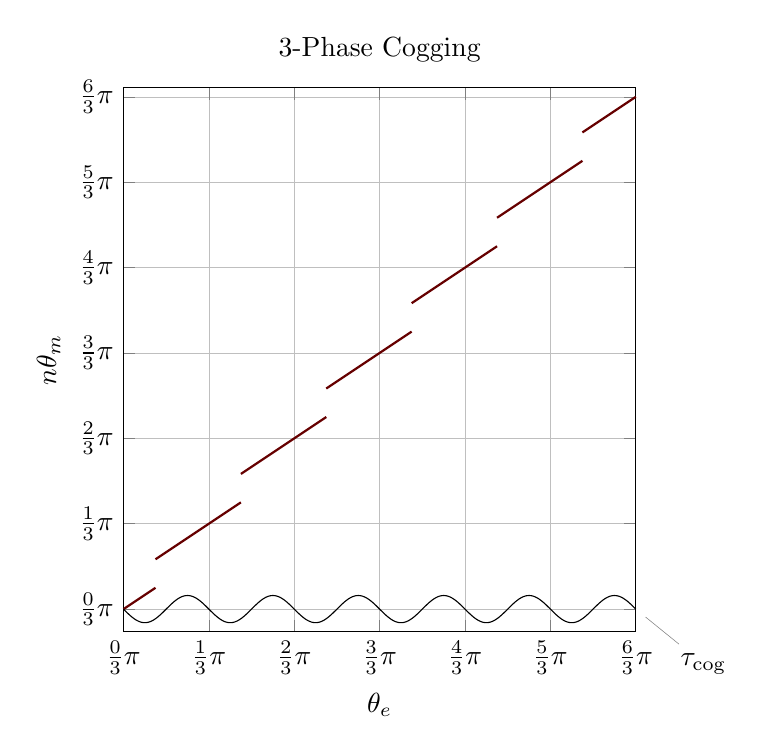
\begin{tikzpicture}[>=latex]
	\begin{axis}[
	width=0.667\textwidth,
	height=0.7\textwidth,
	title=3-Phase Cogging, xlabel={$\theta_e$}, ylabel={$n\theta_m$}, xmin=0, xmax=2*pi, clip=false,
	axis equal=true,
	enlarge x limits=false,
	enlarge y limits=false,
	xmajorgrids,
	ymajorgrids,
	xtick={0,pi/3, 2*pi/3, pi, 4/3*pi, 5/3*pi, 2*pi},
	xticklabels={{$\frac{0}{3}\pi$}, {$\frac{1}{3}\pi$}, {$\frac{2}{3}\pi$}, {$\frac{3}{3}\pi$}, {$\frac{4}{3}\pi$}, {$\frac{5}{3}\pi$}, {$\frac{6}{3}\pi$}},
	ytick={0,pi/3, 2*pi/3, pi, 4/3*pi, 5/3*pi, 2*pi},
	yticklabels={{$\frac{0}{3}\pi$}, {$\frac{1}{3}\pi$}, {$\frac{2}{3}\pi$}, {$\frac{3}{3}\pi$}, {$\frac{4}{3}\pi$}, {$\frac{5}{3}\pi$}, {$\frac{6}{3}\pi$}},
	major y grid style={very thin},
	major x grid style={very thin},
	]
	% phase currents
%	\addplot[domain=0:2*pi,samples=361,red!40!black] {cos(deg(x))} node [pos=1,pin=3:{$A$}] {};
%	\addplot[domain=0:2*pi,samples=361,green!40!black] {cos(deg(x)+120)} node [pos=1,pin=-30:{$B$}] {};
%	\addplot[domain=0:2*pi,samples=361,blue!40!black] {cos(deg(x)+240)} node [pos=1,pin=30:{$C$}] {};

	\addplot[domain=0:0.75*pi/6,samples=361,red!40!black,thick] {0.5/0.75*x};
	\addplot[domain=0.75*pi/6:2.75*pi/6,samples=361,red!40!black,thick] {0.5/0.75*x+0.5/0.75*pi/6};
	\addplot[domain=2.75*pi/6:4.75*pi/6,samples=361,red!40!black,thick] {0.5/0.75*x+1.0/0.75*pi/6};
	\addplot[domain=4.75*pi/6:6.75*pi/6,samples=361,red!40!black,thick] {0.5/0.75*x+1.5/0.75*pi/6};
	\addplot[domain=6.75*pi/6:8.75*pi/6,samples=361,red!40!black,thick] {0.5/0.75*x+2.0/0.75*pi/6};
	\addplot[domain=8.75*pi/6:10.75*pi/6,samples=361,red!40!black,thick] {0.5/0.75*x+2.5/0.75*pi/6};
	\addplot[domain=10.75*pi/6:12.0*pi/6,samples=361,red!40!black,thick] {0.5/0.75*x+3.0/0.75*pi/6};

	% cogging torque
	\addplot[domain=0:2*pi,samples=361,black] {-sin(deg(6*x))/6} node [pos=1,pin=-45:{$\tau_{\textrm{cog}}$}] {};
\end{axis}
\end{tikzpicture}

\caption[Mechanical vs. Electrical position]{Simplified 3-phase cogging during a slow $\theta_e$ sweep. In this plot, it is assumed that the cogging hold is overcome at $3/8$ of the cogging period, without friction and inertia. The main characteristic of this pattern is that the rotor moves slowly close to the stable position, and then jumps once the holding torque is overcome. An important assumption is that $\tau_{\textrm{cog}} << \tau$, and that the difference between electrical and mechanical angle does not grow too large, so that the rotor cannot jump past a stable pole due to inertia.}
\label{fig:cog3-em}
\end{center}
\end{figure}

Doing a slow sweep over $\theta_e$, $n\theta_m$ will show behavior similar to \cref{fig:cog3-em}. We shift our frame of reference to the cogging angle $\theta_c = 6 \theta_e$, for a 3-phase system. Sometime after our phase passes $\theta_c = \pi/2$, the rotor will shoot through the unstable equilibrium between poles, and overshoot the electrical angle towards the next pole. While it is captured by the pole, it will move slower than $\theta_e$ until it jumps again.


When trying to quantify cogging, there are two almost equivalent data points we might be able to measure:
\begin{enumerate}
\item "spring rate" around the equilibrium point,
\item and maximum torque at $\theta_c = \pi/2$.
\end{enumerate}
The unknown quantities effecting the rotor behavior are friction and inertia.

\subsubsection{Linearized Model at Pole}

\begin{figure}[htbp]
\begin{center}
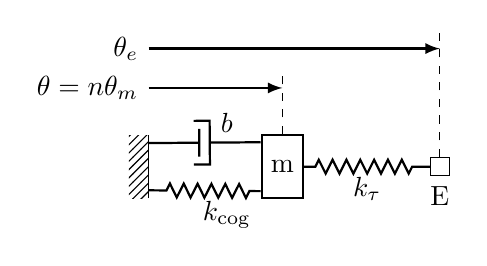
\begin{tikzpicture}[>=latex]
	\tikzstyle{spring}=[thick,decorate,decoration={zigzag,pre length=4,post length=4,segment length=6}]
	\tikzstyle{ground}=[fill,pattern=north east lines,draw=none,minimum width=0.75cm,minimum height=0.3cm,inner sep=0pt,outer sep=0pt]
    \tikzstyle{damper}=[thick,decoration={markings,  
      mark connection node=dmp,
      mark=at position 0.5 with 
      {
        \node (dmp) [thick,inner sep=0pt,transform shape,rotate=-90,minimum width=15pt,minimum height=3pt,draw=none] {};
        \draw [thick] ($(dmp.north east)+(2pt,0)$) -- (dmp.south east) -- (dmp.south west) -- ($(dmp.north west)+(2pt,0)$);
        \draw [thick] ($(dmp.north)+(0,-5pt)$) -- ($(dmp.north)+(0,5pt)$);
      }
    }, decorate]

	% axis
	\draw[thick,->] (-1.5,3.5) node[anchor=east]{$\theta_e$} -- ++( 3.7, 0);
	\draw[thick,->] (-1.5,3.0) node[anchor=east]{$\theta=n\theta_m$} -- ++( 1.7, 0);

	% connecting node
	\node[shape=rectangle,draw,minimum size=0.05cm,minimum height=0.8cm,thick] (A) at (0.2,2) {m};
	\node[shape=rectangle,draw] (B) at (2.2,2) {};
	\draw[dashed] (B.north) -- ( 2.2, 3.7);
	\draw[dashed] (A.north) -- ( 0.2, 3.2);
%	\draw (A.west) node[anchor=east] {M};
	\draw (B.south) node[anchor=north] {E};
    % pin
    \draw[damper,-,thick] ($(A.south west)!0.875!(A.north west)$) -- (-1.5,2.3) node[pos=0.3,above] {$b$};
    \draw[spring,-,thick,decoration={zigzag,segment length=5}] ($(A.south west)!0.125!(A.north west)$) -- (-1.5,1.7) node[pos=0.3,below] {$k_{\mathrm{cog}}$};
    % torque
    \draw[spring,-,thick,decoration={zigzag,segment length=5}] (A.east) -- (B.west) node[pos=0.5,below] {$k_{\tau}$};
%   	\draw[->] (-3,0) -- (3,0); % node[anchor=south west] {$\mathbf{\mu}$};
	% anchor
	\draw (-1.5,2.4) -- ++( 0, -0.8);
	\fill[ground] (-1.5,2.4) -- ++( 0, -0.8) -- ++( -0.25, 0) -- ++( 0, 0.8) -- cycle;

\end{tikzpicture}
\caption[Equilibrium Cogging]{Linear dynamic cogging model around the stable equilibrium. The mechanical rotor can be thought of as a dampened spring mass system, with dampening towards the fixed pole, and a spring to the electrical phase. With the rotor close to the pole, and the torque angle small, both the cogging torque and motor torque can be approximated as linear springs.}
\label{fig:cogeq}
\end{center}
\end{figure}

Around the equilibrium point, a simplified dynamic model might look like \cref{fig:cogeq}. The system equation is 
\begin{gather}
\begin{aligned}
m \ddot{\theta} &= - k_{\textrm{cog}} \theta - k_{\tau} \left(\theta - \theta_e \right) - b \dot{\theta}, \\
m \ddot{\theta} &= - \left(k_{\textrm{cog}} + k_{\tau} \right) \theta - b \dot{\theta} + k_{\tau} \theta_e,
\end{aligned}
\end{gather}
which is equivalent to the standard damped mass-spring model. It might be possible to measure the natural oscillation frequency $\omega_n = \sqrt{\frac{k}{m}}$, where $k=k_{\textrm{cog}} + k_{\tau}$. For a dynamic characterization, we could change $k_{\tau}$ by changing the motor current, and see how the oscillation frequency changes. However, having to measure motor position during a high frequency oscillation for this isn't ideal.

Statically, and in the absence of friction, the system reduces to 
\begin{gather}
\begin{aligned}
0 &= - \left(k_{\textrm{cog}} + k_{\tau} \right) \theta + k_{\tau} \theta_e, \\
k_{\textrm{cog}} &= k_{\tau} \frac{\theta_e - \theta }{\theta} .
\end{aligned}
\end{gather}
This might be easier to measure reliably, though we are constrained to a small actuation angle, and thus limited by encoder resolution.

\subsection{Practical Analysis}

\subsubsection{Stepper Motor}

Let's start with a stepper motor as specified in \cref{tab:17hs16} around zero speed. This means the $E$ component is zero, so the available voltage is $U_d = U - R i$. The motor has a resistance of $R=\unit{1.1}{\ohm}$, an inductance of $L=\unit{2.6}{\milli\henry}$ for a $\unit{2}{\ampere}$ rated current. Assuming a $U=\unit{24}{\volt}$ bus voltage,
\begin{gather}
\begin{aligned}
\frac{\partial \imath}{\partial t} = \frac{\unit{24}{\volt}}{\unit{2.6}{\milli\henry}} = \unit{9.231}{\kilo\ampere\per\second}.
\end{aligned}
\end{gather}
Assuming the cogging torque is 1/3rd of nominal torque, we would need a change of \unit{0.667}{\ampere}, which would take
\begin{gather}
\begin{aligned}
{\partial t} = \frac{\unit{0.667}{\ampere}}{\unit{9.231}{\kilo\ampere\per\second}} = \unit{72.26}{\micro\second}.
\end{aligned}
\end{gather}
or a corresponding electrical system frequency of $f_{\mathrm{cog}} = 1 / 2 \pi \partial t = \unit{2.2}{\kilo\hertz}$.

\subsubsection{BLDC Motor}

For the BLDC as described in \cref{tab:42blf01}, a $R + R$ resistance of \unit{2.36}{\ohm} was measured by supplying \unit{1}{\volt} and measuring \unit{0.423}{\ampere}, while firmware measures $R + R \parallel R$ at \unit{\sim 2.55}{\ohm}.


\appendix

\section{Sinusiodal Mixing}

When mixing two sine waves with $\theta$ and $\varphi$ phases, the equation can be transformed from multiplicative to additive
\begin{gather}
\begin{aligned}
\cos \theta \cos \varphi &= \frac{\cos (\theta - \varphi) + \cos (\theta + \varphi)}{2} \\
\sin \theta \cos \varphi &= \frac{\sin (\theta - \varphi) + \sin (\theta + \varphi)}{2}
\end{aligned}
\end{gather}
which, when the two phases have the same frequency $\lambda = \theta - \varphi$ apart becomes
\begin{gather}
\begin{aligned}
\cos \theta \cos (\theta - \lambda) &= \frac{\cos (\lambda)}{2} + \frac{\cos (2 \theta - \lambda)}{2} \\
\sin \theta \cos (\theta - \lambda) &= \frac{\sin (\lambda)}{2} + \frac{\sin (2 \theta - \lambda)}{2}
\end{aligned}
\end{gather}
which is a DC and a double frequency component. The DC component $f (\lambda)  / 2$ can be used to determine the phase shift.

\section{Linear Regression}

\subsection{Simple Linear Regression}

Simple linear regression is based on a linear model 
\begin{gather}
\begin{aligned}
y &= a + b x
\end{aligned}
\end{gather}
and solves for $a$ and $b$ using a least-squares metric on the sample data. Each sample for $(x_i,y_i)$ is of the form
\begin{gather}
\begin{aligned}
y_i &= a + b x_i + \varepsilon_i
\end{aligned}
\end{gather}
and we try to minimize
\begin{gather}
\begin{aligned}
\min Q(a,b) \quad \mathrm{for} \ Q(a,b) = \sum (y_i - a - b x_i)^2
\end{aligned}
\end{gather}

The estimated coefficients $\hat{a}, \hat{b}$ can then be computed as
\begin{gather}
\begin{aligned}
\hat{b} &= \frac{\sum{(x_i-\bar{x})(y_i-\bar{y})}}{\sum{(x_i - \bar{x})^2}} \\
\hat{a} &= \bar{y} - \hat{b} \bar{x}
\end{aligned}
\end{gather}

\subsection{Moore-Penrose Inverse with SVD}

The Moore-Penrose Inverse $A^+$ of a matrix $A$ is a generalized least-squares inverse of non-square matrices of full rank. 

One numerically efficient method of computing it is by Singular Value Decomposition, which if $A=U\Sigma V^*$, then $A^+=U^*\Sigma^+V$, where $\Sigma$ is a diagonal rectangular matrix and $\Sigma^+$ is computed by taking the inverse of each diagonal element, or zero if the element is smaller than
\begin{gather}
\begin{aligned}
\mathrm{tol} = \varepsilon \cdot \max(m,n) \cdot \max(\Sigma)
\end{aligned}
\end{gather}


\section{Nominal Motor Parameters}
\begin{table}[htbp]
\caption{Stepper Motor 17HS16-2004S-C2.}
\begin{center}
\begin{tabular}{llp{0.5\textwidth}} \toprule
 Parameter & Value & Comment \\
\midrule
Configuration & Bipolar & \\
Step Angle & \unit{1.8}{\degree} & \\
Holding Torque & \unit{0.45}{\newton\meter} & \\
Inductance & \unit{2.6}{\milli\henry} $\pm \unit{20}{\%}$& \\
Resistance & \unit{1.1}{\ohm} $\pm \unit{10}{\%}$ & \\
Rated Current & \unit{2}{\ampere} & \\
Rotor Intertia & \unit{54}{\gram\cdot\centi\meter\squared} & \\
\bottomrule
\end{tabular}
\end{center}
\label{tab:17hs16}
\end{table}%

\begin{table}[htbp]
\caption{BLDC Longs-Motor 42BLF01}
\begin{center}
\begin{tabular}{llp{0.5\textwidth}} \toprule
 Parameter & Value & Comment \\
\midrule
Configuration & Star & \\
Poles & \unit{8}{} & \\
Phases & \unit{3}{} & \\
Holding Torque & \unit{0.063}{\newton\meter} & \\
Peak Torque & \unit{0.18}{\newton\meter} & \\
LtL Inductance & \unit{0.54}{\milli\henry} & \\
LtL Resistance & \unit{1.8}{\ohm} & \\
Peak Current & \unit{4.6}{\ampere} & \\
Rotor Intertia & \unit{24}{\gram\cdot\centi\meter\squared} & \\
BEMF & \unit{4.4}{\volt\per\kilo RPM} & \\
\bottomrule
\end{tabular}
\end{center}
\label{tab:42blf01}
\end{table}%

\section{Open Source Servo Control Survey}

A handful of open source projects exist.

\begin{table}[htbp]
\caption{Open Source Servo Driver Comparison.}
\begin{center}
\begin{tabular}{lrrrrrr} \toprule
 Name & \multicolumn{2}{c}{$U_{\textrm{bus}}$} & $I_{\textrm{nom}}$ & $I_{\textrm{peak}}$ & $f_{\textrm{PWM}}$ & $f_{\textrm{ctrl}}$\\
\midrule
STM32N17   & \unit{12}{\volt} & \unit{48}{\volt}  & \unit{8}{\ampere}  & \unit{?}{\ampere}   & \unit{50}{\kilo\hertz} & \unit{16.7}{\kilo\hertz}\\
Mechaduino & \unit{9}{\volt}  & \unit{25}{\volt}  & \unit{2}{\ampere}  & \unit{2}{\ampere}   & \unit{\sim 30}{\kilo\hertz}  & \unit{?}{\kilo\hertz}\\
ODrive     & \unit{12}{\volt} & \unit{48}{\volt}  & \unit{80}{\ampere} & \unit{120}{\ampere} & \unit{24}{\kilo\hertz}  & \unit{1}{\kilo\hertz}\\
STMBL      & \unit{?}{\volt}  & \unit{450}{\volt} & \unit{8}{\ampere}  & \unit{16}{\ampere}  & \unit{20}{\kilo\hertz}  & \unit{?}{\kilo\hertz}\\
Moteus R4.3 & \unit{12}{\volt}  & \unit{34}{\volt} & \unit{?}{\ampere}  & \unit{100}{\ampere}  & \unit{40}{\kilo\hertz}  & \unit{40}{\kilo\hertz}\\
MicroDriver v2 & \unit{4.4?}{\volt}  & \unit{45?}{\volt} & \unit{?}{\ampere}  & \unit{?}{\ampere}  & \unit{?}{\kilo\hertz}  & \unit{?}{\kilo\hertz}\\
\bottomrule
\end{tabular}
\end{center}
\label{tab:osh}
\end{table}%

\subsection{Mechaduino}

The Mechaduino was the original inspiration for this project. It uses an M0+ MCU, and a A4954 Dual H-Bridge, thus it is only suitable for low-powered 2 phase motors with up to \unit{2}{\ampere} per phase.

The A4954 uses a fixed off-time chopper for current control with \unit{25}{\micro\second} off-time.

The Mechaduino fits on the back of NEMA-17 size stepper motor, and the on-board magnetic encoder allows closed-loop operation without additional hardware.

\subsection{ODrive}

The ODrive is a dual motor servo controller and driver, with up to \unit{48}{\volt} bus voltage and up to \unit{120}{A} peak and \unit{80}{A} continuous current with active cooling. The servo control loop runs \unit{1}{\kilo\hertz}.

The ODrive primarily targets BLDC motors instead of industrial, high-voltage servo motors.

\subsection{STMBL}

STMBL uses the IRAMX16UP60A integrated driver IC\footnote{newer replacement eg. IM393X6FXKLA1}, which supports a high bus voltage of \unit{450}{\volt}, but only a \unit{20}{\kilo\hertz} modulation frequency.

\subsection{Moteus R4.3}

The Moteus controller uses an STM32G4 as its MCU and a DRV8323 as the gate driver. It is designed to be motor-mounted, and has an AS5047 encoder on the back for direct position measurement.

The control scheme is a classical PI/PID cascade controller for torque, speed, and position. 

\subsection{Open Robot Harware Initiative MicroDriver v2}

The MicroDriver is based on a TMS320 DSP.

\section{Higher Voltage/Power considerations}

Exceeding the realm of ca. \unit{50-100}{\volt} bus voltage, 
\begin{enumerate}
\item fully integrated 3-phase gate bridge drivers are no longer available, and discrete components have to be used for the high-side drivers (eg. UCC21521);
\item power transistors change significantly in characteristic with increased switching losses and higher power dissipation;
\item inductive voltage spikes become a larger concern.
\end{enumerate}



\nocite{*}

%\bibliographystyle{ieeetr}
%\bibliography{n17-servo-design}
\printbibliography


\end{document}


